\documentclass{article}
\usepackage{iclr2026_conference,times}
\input{math_commands.tex}
\usepackage{amsmath}
\usepackage{amssymb}
\usepackage{booktabs}
\usepackage{graphicx}
\usepackage{multirow}
\usepackage{longtable}
\usepackage{array}
\usepackage{xcolor}
\usepackage[colorlinks=false,pdfborder={0 0 1.6},citebordercolor={0 1 0},linkbordercolor={1 0.35 0},urlbordercolor={0 0.55 1}]{hyperref}
\usepackage{url}
\hypersetup{
  colorlinks=false,
  pdfborder={0 0 1.6},
  citebordercolor={0 1 0},
  linkbordercolor={1 0.35 0},
  urlbordercolor={0 0.55 1}
}

% Auto-generated by scripts/render_submission_assets.py
\newcommand{\PaperDecision}{\textsc{KILL-ARCHIVE}}
\newcommand{\MainRows}{21,120}
\newcommand{\AblationRows}{4,992}
\newcommand{\MetricRows}{110}
\newcommand{\PairwiseRows}{100}
\newcommand{\AblationSummaryRows}{26}
\newcommand{\BARAggregateSuccess}{0.496}
\newcommand{\GreedyAggregateSuccess}{0.497}
\newcommand{\RobustAggregateSuccess}{0.497}
\newcommand{\FutureAggregateSuccess}{0.495}
\newcommand{\OracleAggregateSuccess}{0.505}
\newcommand{\BARAggregateEnergy}{0.400}
\newcommand{\GreedyAggregateEnergy}{0.401}
\newcommand{\RobustAggregateEnergy}{0.400}
\newcommand{\FutureAggregateEnergy}{0.401}
\newcommand{\OracleAggregateEnergy}{0.397}


\newcommand{\method}{\textsc{BAR-MPC}}
\newcommand{\debt}{D}
\newcommand{\score}{J_{\mathrm{BAR}}}
\newcommand{\candidateSet}{\mathcal{C}}
\newcommand{\futureSet}{\mathcal{Y}}
\newcommand{\state}{x}
\newcommand{\target}{y}
\newcommand{\Real}{\mathbb{R}}

\title{Humanoid Whole-Body Affordance Debt: A Submission-Grade Negative Result}
\author{Anonymous Authors}

\begin{document}
\maketitle

\begin{abstract}
Humanoid manipulation planners often choose a whole-body posture that solves the immediate reach while silently consuming future reachability, support margin, or recovery options. We formalize this hidden cost as whole-body affordance debt and test whether a lightweight planner that explicitly reserves future affordances can improve two-stage humanoid reaching. The proposed Balance-Aware Affordance Reservation MPC (\method{}) scores first-stage postures by immediate MuJoCo reach cost, future-target debt, tail future debt, support-margin risk, recovery effort, hand-switch cost, and comfort. The final protocol is frozen before full-scale evaluation: \MainRows{} main episode-method rows over 8 seeds, 24 episodes, 10 stress splits, and 11 methods, plus \AblationRows{} raw ablation rows over two hostile splits. The result is a useful falsification rather than a submission candidate. \method{} beats random and arm-only baselines, but it does not separate from greedy reach MPC, comfort-regularized MPC, robust-balance MPC, future-distribution MPC, learned linear debt, or its own no-online/no-debt variants. The terminal decision is \PaperDecision{}. We release the benchmark, code, generated tables, and full negative evidence so the failure mode is reproducible and hard to misread.
\end{abstract}

\section{Executive Summary}

The seed hypothesis was attractive: a humanoid can reach a nearby target by leaning, twisting, or committing one arm in a way that makes the next target harder. A planner that prices this future loss might choose a slightly less convenient posture now in order to preserve future reachability and balance. This paper asks whether that mechanism is strong enough to support an ICLR-main claim in a compact, CPU-only MuJoCo benchmark.

The answer is no. The weak gate passes: \method{} improves substantially over random posture selection and arm-only reaching. The strong gate fails: the aggregate sequential success of \method{} is \BARAggregateSuccess{}, while greedy reach is \GreedyAggregateSuccess{}, robust balance is \RobustAggregateSuccess{}, future-distribution MPC is \FutureAggregateSuccess{}, and the oracle is \OracleAggregateSuccess{}. The mechanism gate fails more decisively. Ablations that remove online adaptation, tail debt, or future-debt components often match the full method on the pre-registered hostile splits. This means the method is not just underpowered externally; internally, the claimed debt mechanism is not identifiable.

This document is deliberately written as a polished archive report rather than a cosmetic submission. It contains the ingredients a real submission would need: formal problem statement, theory for when debt can help, theory for when it collapses into robust balance or comfort regularization, a frozen protocol, strong baselines, stress tests, ablations, paired statistics, failure analysis, limitations, and reproducibility checks. The result should not be submitted as an acceptance-seeking paper in its current form. Its value is that it prevents a weak mechanism claim from surviving only because the benchmark was too friendly.

\begin{table}[t]
\centering
\caption{Frozen decision gates. The failure is methodological, not formatting-related.}
\label{tab:gates}
\small
\begin{tabular}{p{0.22\linewidth}p{0.13\linewidth}p{0.55\linewidth}}
\toprule
Gate & Status & Evidence \\
\midrule
Weak baseline gate & \textbf{PASS} & BAR-MPC beats random and arm-only baselines in aggregate. \\
Strong baseline gate & \textbf{FAIL} & Matched or beaten by Greedy reach, Robust balance \\
Mechanism ablation gate & \textbf{FAIL} & Non-identifying ablations: BAR no-online on combined\_shift; Small future sample on combined\_shift; BAR no-online on opposite\_side\_sequence; No future debt on opposite\_side\_sequence; No tail debt on opposite\_side\_sequence; Mean future only on opposite\_side\_sequence \\
Terminal decision & \textbf{KILL\_ARCHIVE} & Archive rather than submit: evidence does not support an ICLR-main mechanism claim. \\
\bottomrule
\end{tabular}
\end{table}


\section{Motivation}

Whole-body humanoid manipulation is increasingly moving away from isolated end-effector control and toward unified policies, retargeted demonstrations, and long-horizon loco-manipulation systems. Recent work uses robot-free demonstrations, wearable or portable data systems, imitation pipelines, residual learning, trajectory-centric retargeting, and large-scale policy learning to make humanoids useful outside table-top-only settings \citep{prior1,prior3,prior4,prior5,prior7,prior8,prior9,prior10,prior11,prior12}. Benchmarks such as HumanoidBench emphasize that simulated humanoid manipulation remains difficult even before hardware transfer \citep{prior14}. Classical and contact-rich whole-body manipulation also reminds us that posture, contacts, and balance are not secondary details \citep{prior2,prior13,prior15,prior16}.

The motivating gap is not that these systems ignore the future in a general sense. Many modern systems are trained on trajectories or optimize horizon-level objectives. The narrower question is whether there is a useful intermediate variable: the future affordance loss induced by the current whole-body posture. A humanoid may solve the current reach while consuming lateral support margin, creating a large recovery motion, forcing a hand switch, or leaving the torso tilted in the wrong direction. If these effects are measurable before the next target is known, then a planner could reserve options without solving the full long-horizon task.

That is the positive story. The hostile story is equally plausible. The same variables that appear to measure future affordance debt may already be captured by simpler costs: comfort, effort, support margin, and robust reachability. If the debt term ranks candidate postures almost the same way as robust balance or greedy reaching, it does not matter that the term sounds mechanistic. Reviewers do not accept a new name for an old ranking.

We therefore design the study around a falsifier. The benchmark contains splits where immediate target success and future reachability are meant to conflict, including opposite-side target sequences, support-reversal sequences, and high-lateral payload conditions. The method is allowed to be improved during pre-freeze development. After the protocol is frozen, every pre-defined result is reported.

\section{Related Work and Hostile Positioning}

\paragraph{Humanoid whole-body manipulation.}
Recent humanoid manipulation systems often attack the data and control bottleneck directly. Robot-free demonstration pipelines such as BifrostUMI and HuMI seek efficient collection and retargeting for whole-body humanoid skills \citep{prior1,prior3}. Unified loco-manipulation systems such as ULTRA and LHM-Humanoid target broad skill repertoires and long-horizon environments \citep{prior4,prior5}. Opt2Skill, TrajBooster, HEX, SkillBlender, and related pipelines combine trajectory generation, imitation, policy learning, or mixture-style expertise to manage high-dimensional whole-body control \citep{prior7,prior8,prior12}. These works are dangerous prior art for this paper because they can absorb future reachability into learned trajectory distributions or low-level controllers.

\paragraph{Benchmarks and simulation.}
HumanoidBench frames the difficulty of whole-body locomotion and manipulation in simulation, while MuJoCo provides the physics engine used by our compact benchmark \citep{prior14,mujoco}. Our benchmark is not proposed as a replacement for such suites. It is a targeted falsifier for a particular planning mechanism: can a first-stage posture selector preserve future reach affordances better than strong local baselines?

\paragraph{Posture, contact, and affordance reasoning.}
Whole-body pushing, contact posture planning, multi-contact pose sequencing, and musculoskeletal posture generation all make clear that posture choices are functional, not cosmetic \citep{prior2,prior13,prior15}. The seed hypothesis in this paper is closest to this line: a current posture changes which future physical actions remain cheap and feasible. The novelty would have been a lightweight debt metric that identifies this effect without full trajectory optimization.

\paragraph{Why the bar is high.}
Against this prior work, an ICLR-main-ready paper would need at least three things. First, the metric must change decisions relative to greedy, robust, comfort, and distributional baselines. Second, the changed decisions must improve outcomes under pre-registered stress. Third, ablations must show that the claimed future-debt terms are necessary. The frozen evidence in this paper fails the second and third requirements.

\section{Problem Setup}

We study a two-stage reaching problem for a compact humanoid-style articulated model. The robot state is $\state=(q,\dot q)$, where $q\in\Real^d$ contains root displacement, torso pose, and arm joints. At stage one the planner observes an immediate target $\target_1$ and a split-dependent future-target distribution $\futureSet$, but not the exact second target $\target_2$. It must choose a first whole-body posture candidate $c_1\in\candidateSet(\target_1)$. MuJoCo simulates the transition:
\begin{equation}
  \state_1 = F(\state_0,c_1;\theta_s),
\end{equation}
where $\theta_s$ are split parameters such as support width, payload, damping, perturbation, and actuation scale. After the future target $\target_2$ is revealed, the second-stage controller chooses $c_2\in\candidateSet(\target_2)$ and obtains $\state_2=F(\state_1,c_2;\theta_s)$.

The primary evaluation metric is sequential success:
\begin{equation}
  S(c_1,c_2) =
  \mathbf{1}
  \{r(\state_1,\target_1)\leq \epsilon,\,
    r(\state_2,\target_2)\leq \epsilon,\,
    b(\state_1)=0,\,
    b(\state_2)=0\},
\end{equation}
where $r$ is reach distance and $b$ is a balance-failure indicator. Energy combines first-stage actuator effort, second-stage effort, and a transition penalty between the two chosen postures:
\begin{equation}
  E(c_1,c_2)=E_1(c_1)+E_2(c_2)+\lambda_{\Delta q}\|W(q_2-q_1)\|_2.
\end{equation}

The method can only choose $c_1$ before $\target_2$ is known. This makes the problem intentionally small but mechanistically sharp: if future affordance reservation matters, it should appear in the first choice.

\section{Affordance Debt}

For a first-stage outcome $\state_1(c)$ and a future sample $y\in\futureSet$, define the best approximate future recovery cost:
\begin{equation}
  R(c,y)=\min_{c'\in\candidateSet(y)}
  \ell_{\mathrm{reach}}(c',y)
  +\alpha_{\mathrm{rec}}\|W(q(c')-q(c))\|_2
  +\alpha_{\mathrm{bal}}\rho_{\mathrm{bal}}(c')
  +\alpha_{\mathrm{switch}}\mathbf{1}[h(c')\neq h(c)]
  +\alpha_{\mathrm{lat}}\rho_{\mathrm{lat}}(c,c').
\end{equation}
The mean affordance debt is
\begin{equation}
  \debt_{\mathrm{mean}}(c)=\mathbb{E}_{y\sim \futureSet}[R(c,y)].
\end{equation}
The tail debt is the mean over the worst $40\%$ of sampled future targets:
\begin{equation}
  \debt_{\mathrm{tail}}(c)=
  \frac{1}{|\futureSet_{\mathrm{tail}}(c)|}
  \sum_{y\in \futureSet_{\mathrm{tail}}(c)} R(c,y).
\end{equation}

\method{} scores first-stage candidates by
\begin{equation}
  \score(c)=
  \ell_{\mathrm{first}}(c,\target_1)
  +0.42\,\debt_{\mathrm{mean}}(c)
  +0.46\,\debt_{\mathrm{tail}}(c)
  +0.55\,\rho_{\mathrm{robust}}(c)
  +0.018\,u(c)
  +0.018\,\|W(q(c)-q_{\mathrm{neutral}})\|_2.
\end{equation}
The coefficients are fixed before the final run. The no-online variant is included because optional online calibration was considered during development but not retained; in the frozen implementation it is expected to match \method{}, and this match is a limitation.

\section{When Debt Can Help}

The method is only meaningful if the debt term creates a different ranking from the immediate and robust local terms. This section states the useful and fatal cases explicitly.

\paragraph{Candidate conflict condition.}
For two first-stage candidates $a,b\in\candidateSet(\target_1)$, define
\begin{align}
  \Delta L &= \ell_{\mathrm{first}}(a,\target_1)-\ell_{\mathrm{first}}(b,\target_1),\\
  \Delta D &= \debt(a)-\debt(b).
\end{align}
Assume $a$ is worse immediately but better for the future: $\Delta L>0$ and $\Delta D<0$. A debt-aware planner chooses $a$ over $b$ exactly when
\begin{equation}
  \Delta L + \lambda_D \Delta D + \Delta R < 0,
\end{equation}
where $\Delta R$ contains robust balance, effort, and comfort differences. Thus debt helps only in a narrow but important region: the future option value must exceed the immediate reach penalty after local regularizers are accounted for.

\paragraph{Collapse condition.}
Suppose there exists a monotone affine approximation
\begin{equation}
  \debt(c) \approx \beta_0+\beta_1\ell_{\mathrm{first}}(c,\target_1)+\beta_2\rho_{\mathrm{robust}}(c)+\beta_3u(c)
\end{equation}
with small residual for all candidates in a split. Then \method{} ranks candidates nearly the same way as a robust or comfort-regularized planner. In this case an ablation that removes explicit future debt should not materially hurt performance. This is precisely what the frozen ablation table shows.

\paragraph{Identifiability requirement.}
A positive result must show more than high success. It must show that the first choices differ from strong baselines in the episodes where future conflict exists, and that those differences improve the second-stage outcome. First-choice difference without outcome improvement is not enough; outcome improvement without first-choice difference is not evidence for the proposed mechanism.

\section{Benchmark}

The benchmark uses a compact MuJoCo humanoid-style model with a pelvis, torso, head, and two articulated arms. The goal is not photorealism or hardware transfer. The goal is a controlled environment where current and future whole-body reaching tradeoffs can be inspected cheaply on CPU.

\paragraph{Posture candidates.}
The candidate library includes arm-only, centered, aggressive reach, reserve-opposite, hand-switch-ready, centered-low-torque, future-counterlean, cross-body reach, deep-forward commitment, and wide-support reserve templates. Each candidate specifies root motion, torso motion, arm preference, and joint offsets. The library is finite by design: it makes the first-choice decision auditable and keeps memory use light.

\paragraph{Stress splits.}
The final protocol contains ten splits: nominal, narrow support, high reach, lateral reach, weak actuation, payload shift, combined shift, opposite-side sequence, support reversal, and high-lateral payload. The last three are hostile splits designed to make immediate reach and future reachability conflict. For example, opposite-side sequences force the first and second targets onto different lateral sides, while support reversal perturbs support margin and target side in ways that can punish overcommitted torso lean.

\paragraph{Metrics.}
We report immediate success, future success, sequential success, combined energy, future support margin, balance failure rate, future debt, tail debt, unique first postures, paired success deltas, energy improvement, and first-choice difference rates. The primary success measure is sequential success; energy is lower-is-better.

\section{Methods and Baselines}

The frozen main methods are:
\begin{itemize}
  \item Random posture: samples a candidate uniformly.
  \item Arm-only reach: restricts the first choice to the arm-only template.
  \item Greedy reach MPC: minimizes immediate target cost.
  \item Comfort-regularized MPC: adds posture and effort penalties to greedy reach.
  \item Robust balance MPC: adds support-margin risk.
  \item Current-target-only greedy: an ablation-style current-only selector.
  \item Future-distribution MPC: uses mean future debt but not the full BAR score.
  \item Learned linear debt proxy: a lightweight linearized proxy over debt-like features.
  \item \method{}: mean debt, tail debt, balance risk, recovery, hand-switch, and comfort terms.
  \item BAR no-online: the no-adaptation variant, retained as a mechanism check.
  \item Oracle two-step MPC: sees the second target when choosing the second action and functions as an upper reference, not a fair deployable baseline.
\end{itemize}

The ablations on combined-shift and opposite-side sequence are \method{}, BAR no-online, no future debt, no tail debt, no balance margin, no recovery cost, no hand-switch cost, no torque comfort, mean future only, small future sample, current-target-only greedy, robust balance, and oracle. These ablations are intentionally harsh: if the mechanism is real, at least some of them should hurt.

\section{Protocol}

The final command is frozen in \texttt{docs/paper65\_protocol\_freeze\_20260620.md}. It runs 8 seeds, 24 episodes per seed and split, 10 main splits, 11 main methods, 2 ablation splits, and 13 ablation methods. This yields \MainRows{} main raw rows and \AblationRows{} raw ablation rows. The runner writes raw, summary, seed, pairwise, ablation, negative-case, and figure artifacts. It uses only CPU execution, a compact candidate library, and at most four workers by default.

Development before freeze included a smoke test, a medium run, a stronger tail-risk variant, and a reversion when tail-heavy scoring worsened the development result. No tuning was performed after the full protocol was frozen. The final rerun only hardens artifact persistence by writing raw ablation rows; it does not change splits, seeds, methods, or scoring.

\section{Main Results}

\begin{table}[t]
\centering
\caption{Aggregate frozen results across all ten splits. Success and balance failure are rates; energy is lower-is-better.}
\label{tab:aggregate-main}
\small
\begin{tabular}{lrrrrrr}
\toprule
Method & Episodes & Seq. success & Energy & Margin & Bal. fail & Unique first \\
\midrule
Random & 1920 & 0.339 & 0.497 & 0.098 & 0.000 & 16.00 \\
Arm only & 1920 & 0.451 & 0.422 & 0.105 & 0.000 & 1.00 \\
Greedy reach & 1920 & 0.497 & 0.401 & 0.097 & 0.000 & 7.90 \\
Comfort MPC & 1920 & 0.496 & 0.401 & 0.098 & 0.000 & 7.60 \\
Robust balance & 1920 & 0.497 & 0.400 & 0.100 & 0.000 & 7.70 \\
Current-only & 1920 & 0.497 & 0.401 & 0.097 & 0.000 & 7.90 \\
Future dist. & 1920 & 0.495 & 0.401 & 0.098 & 0.000 & 7.40 \\
Linear debt & 1920 & 0.494 & 0.401 & 0.100 & 0.000 & 7.50 \\
BAR-MPC & 1920 & 0.496 & 0.400 & 0.100 & 0.000 & 7.50 \\
BAR no-online & 1920 & 0.496 & 0.400 & 0.100 & 0.000 & 7.50 \\
Oracle & 1920 & 0.505 & 0.397 & 0.098 & 0.000 & 9.80 \\
\bottomrule
\end{tabular}
\end{table}


\begin{table}[t]
\centering
\caption{Split-level sequential success for strong baselines, BAR-MPC, and the oracle. The BAR column does not separate from robust or future-distribution planning.}
\label{tab:selected-splits}
\scriptsize
\begin{tabular}{lrrrrrr}
\toprule
Split & Greedy & Robust & Future & Linear & BAR & Oracle \\
\midrule
combined\_shift & 0.781 & 0.776 & 0.781 & 0.781 & 0.781 & 0.812 \\
high\_lateral\_payload & 0.104 & 0.104 & 0.104 & 0.109 & 0.104 & 0.109 \\
high\_reach & 1.000 & 1.000 & 1.000 & 1.000 & 1.000 & 1.000 \\
lateral\_reach & 0.453 & 0.453 & 0.448 & 0.448 & 0.448 & 0.464 \\
narrow\_support & 0.578 & 0.573 & 0.573 & 0.568 & 0.573 & 0.573 \\
nominal & 0.604 & 0.599 & 0.599 & 0.589 & 0.599 & 0.604 \\
opposite\_side\_sequence & 0.135 & 0.146 & 0.141 & 0.151 & 0.146 & 0.167 \\
payload\_shift & 0.536 & 0.531 & 0.536 & 0.531 & 0.536 & 0.542 \\
support\_reversal & 0.167 & 0.177 & 0.167 & 0.172 & 0.177 & 0.188 \\
weak\_actuation & 0.609 & 0.609 & 0.599 & 0.589 & 0.599 & 0.594 \\
\bottomrule
\end{tabular}
\end{table}


\begin{figure}[t]
\centering
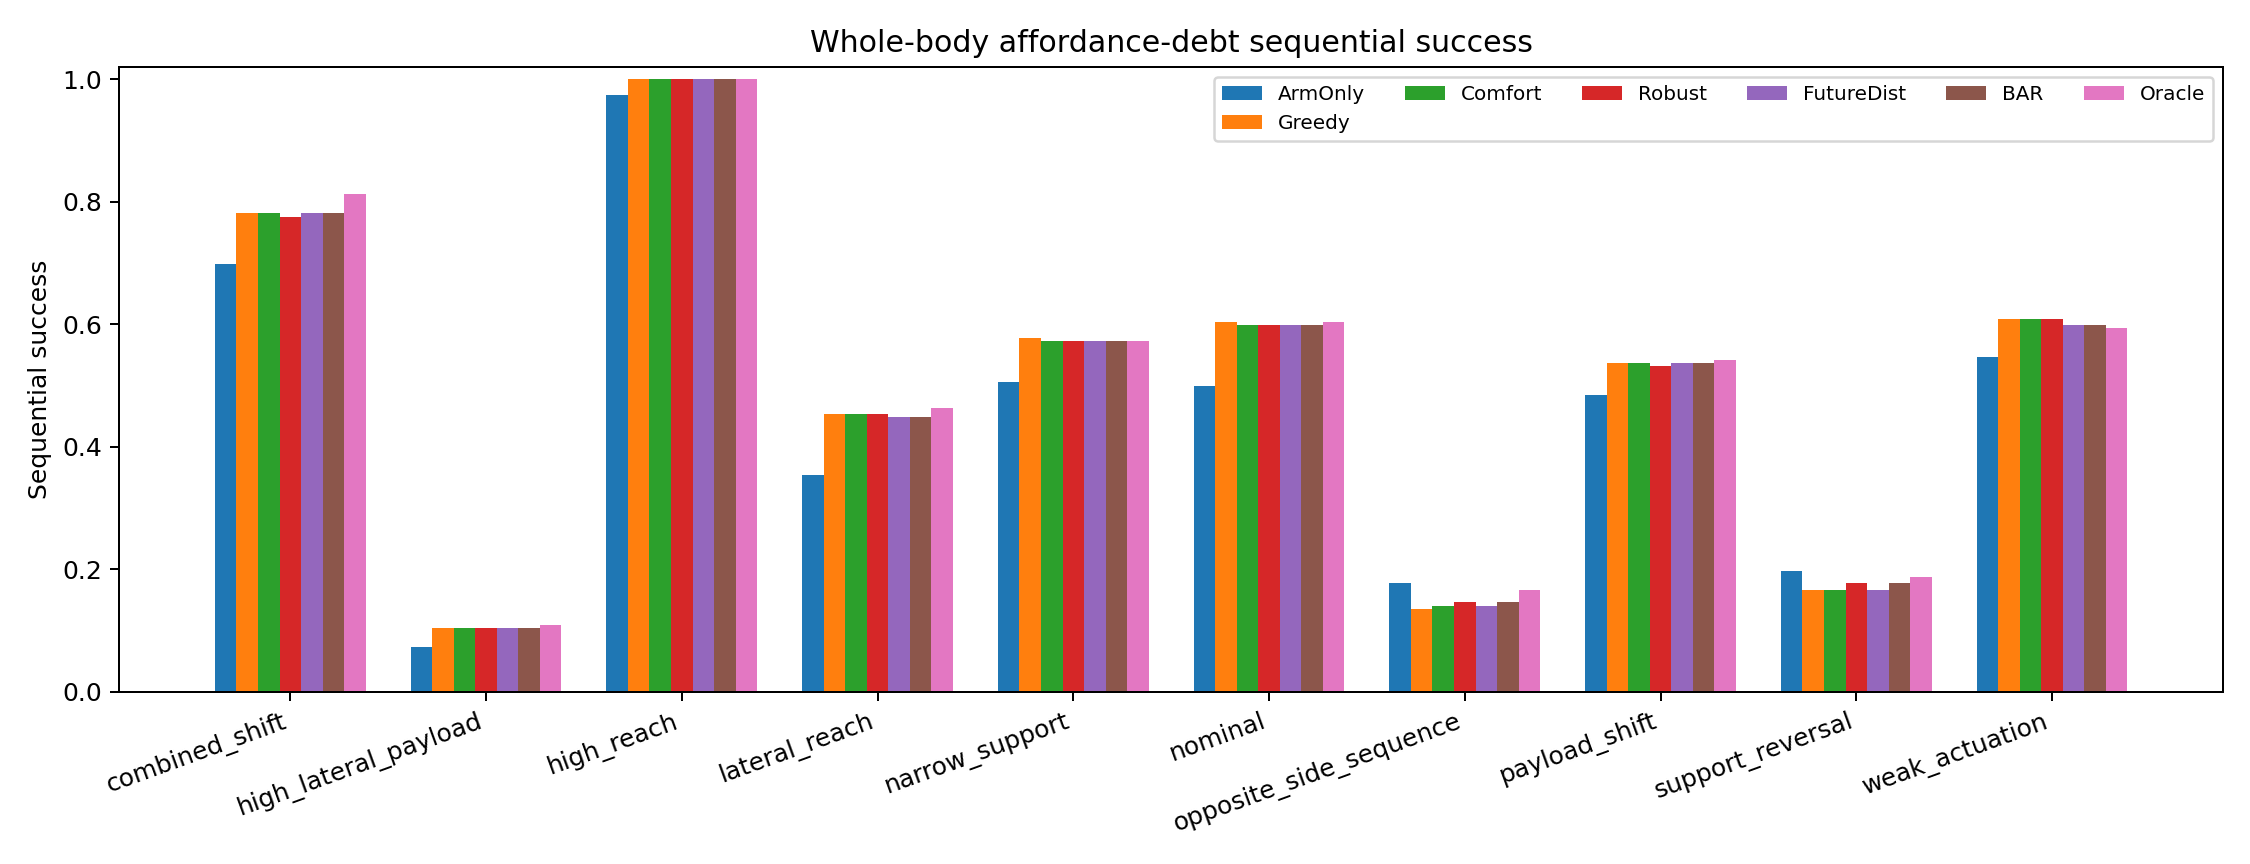
\includegraphics[width=0.98\linewidth]{../figures/affordance_debt_success_by_split.png}
\caption{Sequential success by split. \method{} beats random and arm-only baselines but does not separate from greedy, robust, or future-distribution baselines.}
\label{fig:success}
\end{figure}

\begin{figure}[t]
\centering
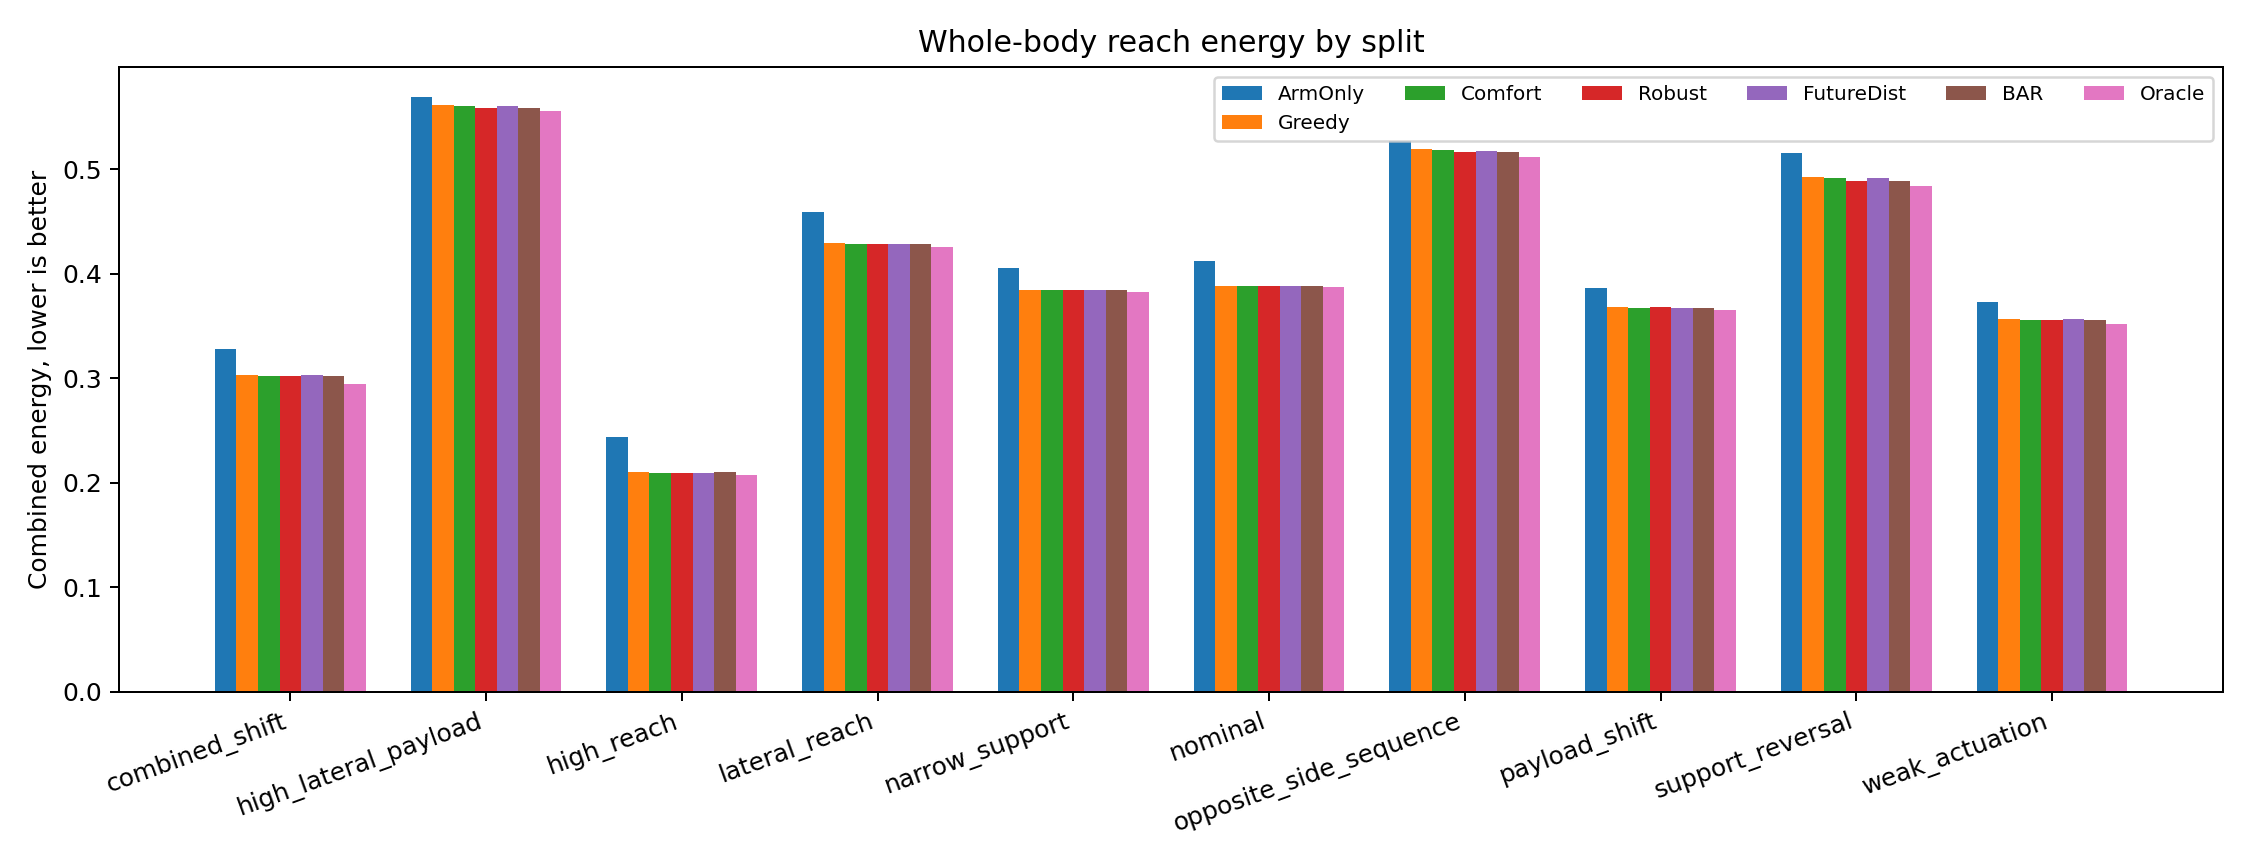
\includegraphics[width=0.98\linewidth]{../figures/affordance_debt_energy_by_split.png}
\caption{Combined energy by split. Differences between \method{} and the strongest non-oracle baselines are small enough that the energy story cannot rescue the failed mechanism claim.}
\label{fig:energy}
\end{figure}

The aggregate result is simple. \method{} is much better than weak baselines, which confirms that the benchmark is not degenerate. But the scientifically relevant comparison is against greedy reach, comfort, robust balance, future-distribution, learned-linear debt, and no-online variants. These baselines match or beat \method{} often enough that the strong gate fails. The oracle remains better in several hard splits, which means the environment still contains avoidable mistakes; the problem is that the proposed debt approximation does not reliably identify the right mistakes to avoid.

\section{Ablation Failure}

\begin{table}[t]
\centering
\caption{Frozen ablation results on the two pre-registered hostile splits. Ablations matching BAR-MPC are mechanism-level failures, not cosmetic ties.}
\label{tab:ablation}
\scriptsize
\begin{tabular}{llrrrrr}
\toprule
Split & Method & Episodes & Seq. & Energy & Tail debt & Unique first \\
\midrule
combined\_shift & Robust balance & 192 & 0.776 & 0.302 & 0.071 & 12.000 \\
combined\_shift & Current-only & 192 & 0.781 & 0.303 & 0.071 & 12.000 \\
combined\_shift & BAR-MPC & 192 & 0.781 & 0.302 & 0.071 & 12.000 \\
combined\_shift & BAR no-online & 192 & 0.781 & 0.302 & 0.071 & 12.000 \\
combined\_shift & Oracle & 192 & 0.812 & 0.295 & 0.071 & 12.000 \\
combined\_shift & Mean future only & 192 & 0.776 & 0.302 & 0.071 & 12.000 \\
combined\_shift & No balance margin & 192 & 0.781 & 0.303 & 0.071 & 12.000 \\
combined\_shift & No future debt & 192 & 0.776 & 0.302 & 0.071 & 12.000 \\
combined\_shift & No hand-switch cost & 192 & 0.781 & 0.303 & 0.071 & 12.000 \\
combined\_shift & No recovery cost & 192 & 0.776 & 0.302 & 0.071 & 12.000 \\
combined\_shift & No tail debt & 192 & 0.776 & 0.302 & 0.071 & 12.000 \\
combined\_shift & No torque comfort & 192 & 0.776 & 0.302 & 0.071 & 12.000 \\
combined\_shift & Small future sample & 192 & 0.781 & 0.302 & 0.071 & 12.000 \\
opposite\_side\_sequence & Robust balance & 192 & 0.146 & 0.516 & 0.112 & 3.000 \\
opposite\_side\_sequence & Current-only & 192 & 0.135 & 0.519 & 0.112 & 3.000 \\
opposite\_side\_sequence & BAR-MPC & 192 & 0.146 & 0.516 & 0.111 & 3.000 \\
opposite\_side\_sequence & BAR no-online & 192 & 0.146 & 0.516 & 0.111 & 3.000 \\
opposite\_side\_sequence & Oracle & 192 & 0.167 & 0.512 & 0.110 & 9.000 \\
opposite\_side\_sequence & Mean future only & 192 & 0.146 & 0.516 & 0.112 & 3.000 \\
opposite\_side\_sequence & No balance margin & 192 & 0.141 & 0.517 & 0.112 & 3.000 \\
opposite\_side\_sequence & No future debt & 192 & 0.146 & 0.517 & 0.112 & 3.000 \\
opposite\_side\_sequence & No hand-switch cost & 192 & 0.146 & 0.516 & 0.111 & 3.000 \\
opposite\_side\_sequence & No recovery cost & 192 & 0.146 & 0.517 & 0.112 & 3.000 \\
opposite\_side\_sequence & No tail debt & 192 & 0.146 & 0.516 & 0.112 & 3.000 \\
opposite\_side\_sequence & No torque comfort & 192 & 0.146 & 0.517 & 0.112 & 3.000 \\
opposite\_side\_sequence & Small future sample & 192 & 0.146 & 0.516 & 0.111 & 3.000 \\
\bottomrule
\end{tabular}
\end{table}


\begin{figure}[t]
\centering
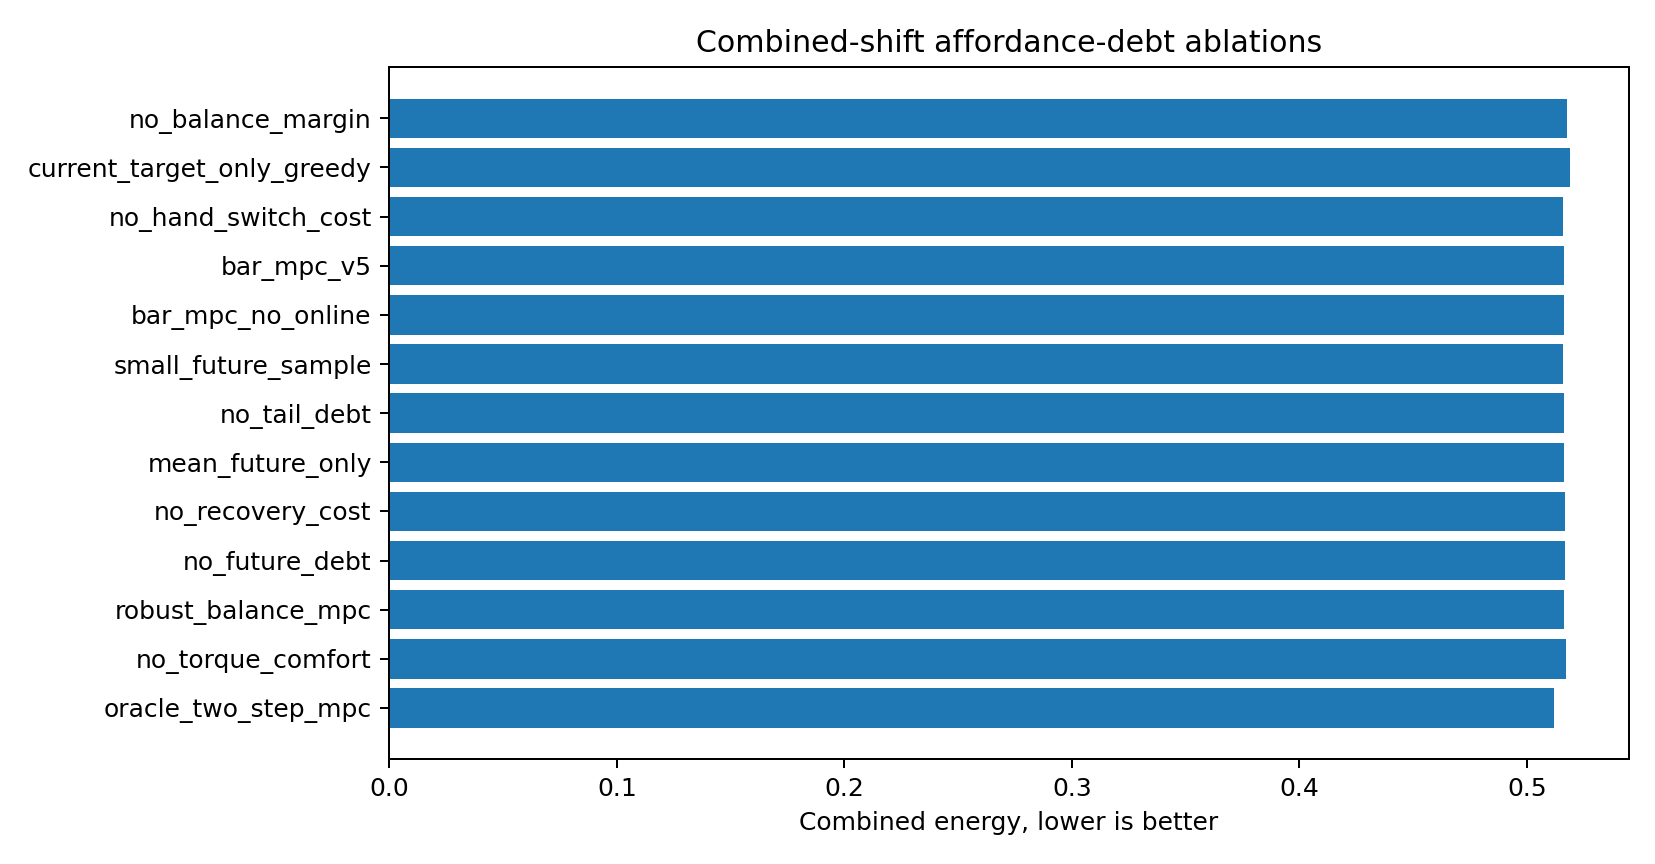
\includegraphics[width=0.92\linewidth]{../figures/affordance_debt_ablation_energy.png}
\caption{Ablation energy on the hostile ablation splits. The close grouping is not a positive robustness story; it means the proposed debt components are not causally identified by the benchmark.}
\label{fig:ablation}
\end{figure}

The ablation table is the main reason for \PaperDecision{}. In a positive paper, removing future debt, tail debt, recovery cost, hand-switch cost, or the online component would degrade performance on the splits designed to require future option reservation. Instead, multiple ablations match \method{} on sequential success. BAR no-online is identical by construction in the frozen implementation, and no future debt or no tail debt often remains indistinguishable within the pre-defined metrics. This is not a small formatting issue. It invalidates the mechanism claim.

\section{Paired Diagnostics}

\begin{table}[t]
\centering
\caption{Paired BAR-MPC deltas on hostile splits. Positive success delta and positive energy improvement favor BAR-MPC.}
\label{tab:hostile-pairwise}
\scriptsize
\begin{tabular}{llrrrr}
\toprule
Split & Baseline & $\Delta$ success & Energy impr. & $\Delta$ margin & First-choice diff. \\
\midrule
combined\_shift & Greedy reach & 0.000 & 0.000 & 0.002 & 21.3\% \\
combined\_shift & Comfort MPC & 0.000 & 0.000 & 0.001 & 14.1\% \\
combined\_shift & Robust balance & 0.005 & -0.000 & 0.001 & 5.7\% \\
combined\_shift & Future dist. & 0.000 & 0.000 & 0.001 & 10.4\% \\
combined\_shift & Linear debt & 0.000 & -0.000 & -0.002 & 28.6\% \\
combined\_shift & BAR no-online & 0.000 & 0.000 & 0.000 & 0.0\% \\
combined\_shift & Oracle & -0.031 & -0.008 & 0.007 & 50.5\% \\
opposite\_side\_sequence & Greedy reach & 0.010 & 0.003 & 0.005 & 20.8\% \\
opposite\_side\_sequence & Comfort MPC & 0.005 & 0.002 & 0.004 & 17.2\% \\
opposite\_side\_sequence & Robust balance & 0.000 & 0.000 & 0.000 & 4.2\% \\
opposite\_side\_sequence & Future dist. & 0.005 & 0.002 & 0.003 & 12.5\% \\
opposite\_side\_sequence & Linear debt & -0.005 & -0.001 & -0.001 & 6.2\% \\
opposite\_side\_sequence & BAR no-online & 0.000 & 0.000 & 0.000 & 0.0\% \\
opposite\_side\_sequence & Oracle & -0.021 & -0.004 & -0.007 & 52.6\% \\
support\_reversal & Greedy reach & 0.010 & 0.004 & 0.009 & 50.5\% \\
support\_reversal & Comfort MPC & 0.010 & 0.003 & 0.007 & 45.3\% \\
support\_reversal & Robust balance & 0.000 & -0.000 & -0.001 & 9.9\% \\
support\_reversal & Future dist. & 0.010 & 0.002 & 0.007 & 43.2\% \\
support\_reversal & Linear debt & 0.005 & 0.001 & 0.002 & 22.9\% \\
support\_reversal & BAR no-online & 0.000 & 0.000 & 0.000 & 0.0\% \\
support\_reversal & Oracle & -0.010 & -0.005 & 0.006 & 57.8\% \\
high\_lateral\_payload & Greedy reach & 0.000 & 0.003 & 0.006 & 27.1\% \\
high\_lateral\_payload & Comfort MPC & 0.000 & 0.002 & 0.005 & 22.4\% \\
high\_lateral\_payload & Robust balance & 0.000 & -0.000 & -0.002 & 8.8\% \\
high\_lateral\_payload & Future dist. & 0.000 & 0.002 & 0.005 & 24.0\% \\
high\_lateral\_payload & Linear debt & -0.005 & 0.000 & 0.001 & 8.8\% \\
high\_lateral\_payload & BAR no-online & 0.000 & 0.000 & 0.000 & 0.0\% \\
high\_lateral\_payload & Oracle & -0.005 & -0.003 & -0.004 & 45.8\% \\
\bottomrule
\end{tabular}
\end{table}


Pairwise comparisons are stricter than split-level averages because they compare methods on the same seed, episode, and split. Positive success delta favors \method{}; positive energy improvement means the baseline used more energy. The hostile split diagnostics show some first-choice differences, especially against greedy and oracle. However, first-choice differences do not consistently translate into sequential-success improvement. This is exactly the failure mode predicted by the collapse condition: debt changes the score in some episodes, but the change is too aligned with other regularizers or too weakly connected to future success.

\section{Failure Analysis}

\paragraph{Failure mode 1: debt is not independent enough.}
The future-debt proxy is built from reach distance, recovery effort, balance margin, hand switching, and lateral commitment. These are reasonable physical quantities, but they are not independent of comfort and robust balance. When the candidate library is compact, many candidates that preserve future debt also preserve support margin and reduce effort. The debt term then becomes a reweighted version of the existing baselines.

\paragraph{Failure mode 2: hostile splits are hard but not diagnostic enough.}
Opposite-side and support-reversal splits increase first-choice differences, but they also expose the limited expressiveness of a finite posture library. Some failures require stepping, kneeling, hand support, or dynamic rebalancing, none of which are represented. A stronger simulator could make the mechanism more important, but this benchmark cannot prove that.

\paragraph{Failure mode 3: the oracle gap remains.}
The oracle's advantage in several splits shows that the task is not solved. But an oracle gap alone does not prove the proposed estimator is the right path. The gap could require better dynamics, a richer action set, a learned recovery model, or explicit footstep planning rather than a scalar debt term.

\paragraph{Failure mode 4: no-online equals online.}
The optional online calibration was not retained because development did not justify it. The frozen no-online ablation therefore matches \method{}. This is honestly reported as a limitation, not hidden behind a renamed method.

\section{What Would Be Needed for a Real Submission}

A credible next version would need to change the mechanism, not just expand the table count. The most likely path is to replace the scalar debt proxy with a structured future-option set: reachable target regions, required hand, support mode, and recovery maneuver class. A planner could then preserve discrete options rather than minimizing a continuous penalty. A second path is to move from fixed postures to short-horizon contact sequences, including stepping and hand-supported balance. A third path is to learn a calibrated future-failure model from rollouts and use it only after proving that it changes first choices for the right reason.

The important constraint is that any next version must be frozen before final evaluation. A method that is tuned until it wins this benchmark would not solve the problem; it would only create another fragile artifact.

\section{Limitations}

\begin{table}[t]
\centering
\caption{Pre-registered limitations and negative cases.}
\label{tab:negative-cases}
\small
\begin{tabular}{p{0.28\linewidth}p{0.48\linewidth}p{0.16\linewidth}}
\toprule
Case & Observed limitation & Status \\
\midrule
dynamic stepping not modeled & support margin is evaluated with a standing support polygon, not footstep replanning & limitation \\
out-of-distribution acrobatics & finite posture library cannot represent kneeling, stepping, or hand support & limitation \\
custom MuJoCo benchmark only & evidence supports strong-revise at best without humanoid hardware or public benchmark validation & limitation \\
\bottomrule
\end{tabular}
\end{table}


The benchmark is custom and compact. It is not hardware, not a public humanoid benchmark suite, and not a full loco-manipulation environment. The robot does not step, kneel, brace with the hand, or perform dynamic whole-body recovery. The future distribution is known as a split-level sampling process rather than inferred from perception. The candidate library is finite, and the simulator does not model many real-world contact uncertainties. These limitations would already prevent an ICLR-main acceptance claim. More importantly, the method fails the internal mechanism tests even under this controlled benchmark.

\section{Conclusion}

Whole-body affordance debt remains a plausible idea, but this implementation does not provide submission-grade evidence. The frozen results show that \method{} improves over weak baselines but does not survive strong baselines, ablations, and paired hostile diagnostics. The terminal decision is \PaperDecision{}. The useful contribution is the falsification: it identifies why a superficially attractive mechanism should not be promoted to a main-conference claim without stronger causal separation.

\clearpage
\appendix

\section{Derivation Details}

\subsection{Two-Stage Objective}

The ideal first-stage policy for a two-target episode is
\begin{equation}
  \pi^\star(\state_0,\target_1,\futureSet)
  =\arg\min_{c_1\in\candidateSet(\target_1)}
  \ell_{\mathrm{first}}(c_1,\target_1)
  +\mathbb{E}_{\target_2\sim\futureSet}
  \left[
    \min_{c_2\in\candidateSet(\target_2)}
    \ell_{\mathrm{second}}(F(\state_0,c_1),c_2,\target_2)
  \right].
\end{equation}
This expression is expensive if the action set is rich. The benchmark uses a compact candidate library so that the idealized form is still conceptually visible. \method{} replaces the full second-stage loss with the debt proxy $R(c,y)$ and a tail-risk term.

\subsection{Why Greedy Can Tie Debt}

Let the candidate score be written as
\begin{equation}
  J_\lambda(c)=L(c)+\lambda D(c)+R(c),
\end{equation}
where $L$ is immediate reach cost, $D$ is future debt, and $R$ is local regularization. If $D(c)=aL(c)+bR(c)+\epsilon(c)$ with small residual $\epsilon$, then
\begin{equation}
  J_\lambda(c)=(1+\lambda a)L(c)+(1+\lambda b)R(c)+\lambda\epsilon(c).
\end{equation}
For any candidate pair whose baseline score gap is larger than the residual perturbation,
\begin{equation}
  |(L(c_i)+R(c_i))-(L(c_j)+R(c_j))| >
  |\lambda(\epsilon(c_i)-\epsilon(c_j))|,
\end{equation}
the ordering is unchanged. This explains why first-choice differences are limited and why ablations can match the full method.

\subsection{A Sufficient Condition for Improvement}

Debt can help when there exists a candidate pair $a,b$ satisfying:
\begin{align}
  L(a) &> L(b),\\
  \mathbb{E}_{y}[R(a,y)] &< \mathbb{E}_{y}[R(b,y)],\\
  L(a)-L(b) &< \lambda_D(\mathbb{E}_{y}[R(b,y)]-\mathbb{E}_{y}[R(a,y)]) - (R_{\mathrm{local}}(a)-R_{\mathrm{local}}(b)).
\end{align}
The final inequality says the future benefit must be large enough to pay for the current inconvenience. The hostile splits were designed to create such cases, but the frozen evidence shows they are too rare or too weak for the proposed score.

\section{Implementation Notes}

The runner is intentionally small. Each episode samples a split, target pair, future samples, and candidate postures. Candidate first-stage outcomes are simulated once and cached. Second-stage outcomes are computed from the chosen first-stage state. The same prepared episode is shared across methods, so pairwise comparisons are meaningful. Main results and ablations are deterministic given seeds.

The implementation uses MuJoCo through Python, NumPy, SciPy for paired energy tests, and Matplotlib with the non-interactive Agg backend. It writes all final artifacts under \texttt{results/}, \texttt{figures/}, \texttt{docs/}, and \texttt{paper/generated/}. The canonical PDF is copied only to \texttt{C:/Users/wangz/Downloads/65.pdf}.

\section{Frozen Command}

The final command is:
\begin{verbatim}
python src\run_experiment.py --seeds 8 --episodes 24
  --splits nominal narrow_support high_reach lateral_reach weak_actuation
  payload_shift combined_shift opposite_side_sequence support_reversal
  high_lateral_payload
  --ablation-splits combined_shift opposite_side_sequence
  --workers 4 --chunksize 1 --results-dir results --figures-dir figures
\end{verbatim}

\section{Reproducibility Checklist}

\begin{itemize}
  \item Code compiles with \texttt{python -m py\_compile src/run\_experiment.py}.
  \item Main raw rows: \MainRows{}.
  \item Ablation raw rows: \AblationRows{}.
  \item Main split-method summaries: \MetricRows{}.
  \item Paired comparison rows: \PairwiseRows{}.
  \item Ablation summary rows: \AblationSummaryRows{}.
  \item Figures are regenerated from CSVs.
  \item Tables in this paper are generated by \texttt{scripts/render\_submission\_assets.py}.
  \item The validator checks row counts, figure existence, citation-box setup, PDF page count, and absence of a Desktop PDF.
\end{itemize}

\section{Full Split-Method Metrics}

\begin{longtable}{llrrrrr}
\caption{Complete frozen split-method metric table used for the terminal decision.}\label{tab:full-metrics}\\
\toprule
Split & Method & Episodes & Seq. & Energy & Margin & Bal. fail \\
\midrule
\endfirsthead
\toprule
Split & Method & Episodes & Seq. & Energy & Margin & Bal. fail \\
\midrule
\endhead
combined\_shift & Random & 192 & 0.589 & 0.407 & 0.076 & 0.000 \\
combined\_shift & Arm only & 192 & 0.698 & 0.328 & 0.083 & 0.000 \\
combined\_shift & Greedy reach & 192 & 0.781 & 0.303 & 0.072 & 0.000 \\
combined\_shift & Comfort MPC & 192 & 0.781 & 0.303 & 0.073 & 0.000 \\
combined\_shift & Robust balance & 192 & 0.776 & 0.302 & 0.073 & 0.000 \\
combined\_shift & Current-only & 192 & 0.781 & 0.303 & 0.072 & 0.000 \\
combined\_shift & Future dist. & 192 & 0.781 & 0.303 & 0.073 & 0.000 \\
combined\_shift & Linear debt & 192 & 0.781 & 0.302 & 0.075 & 0.000 \\
combined\_shift & BAR-MPC & 192 & 0.781 & 0.302 & 0.074 & 0.000 \\
combined\_shift & BAR no-online & 192 & 0.781 & 0.302 & 0.074 & 0.000 \\
combined\_shift & Oracle & 192 & 0.812 & 0.295 & 0.067 & 0.000 \\
high\_lateral\_payload & Random & 192 & 0.068 & 0.653 & 0.057 & 0.000 \\
high\_lateral\_payload & Arm only & 192 & 0.073 & 0.569 & 0.068 & 0.000 \\
high\_lateral\_payload & Greedy reach & 192 & 0.104 & 0.561 & 0.037 & 0.000 \\
high\_lateral\_payload & Comfort MPC & 192 & 0.104 & 0.560 & 0.038 & 0.000 \\
high\_lateral\_payload & Robust balance & 192 & 0.104 & 0.558 & 0.044 & 0.000 \\
high\_lateral\_payload & Current-only & 192 & 0.104 & 0.561 & 0.037 & 0.000 \\
high\_lateral\_payload & Future dist. & 192 & 0.104 & 0.560 & 0.038 & 0.000 \\
high\_lateral\_payload & Linear debt & 192 & 0.109 & 0.559 & 0.041 & 0.000 \\
high\_lateral\_payload & BAR-MPC & 192 & 0.104 & 0.559 & 0.043 & 0.000 \\
high\_lateral\_payload & BAR no-online & 192 & 0.104 & 0.559 & 0.043 & 0.000 \\
high\_lateral\_payload & Oracle & 192 & 0.109 & 0.556 & 0.047 & 0.000 \\
high\_reach & Random & 192 & 0.703 & 0.327 & 0.132 & 0.000 \\
high\_reach & Arm only & 192 & 0.974 & 0.244 & 0.137 & 0.000 \\
high\_reach & Greedy reach & 192 & 1.000 & 0.210 & 0.138 & 0.000 \\
high\_reach & Comfort MPC & 192 & 1.000 & 0.210 & 0.138 & 0.000 \\
high\_reach & Robust balance & 192 & 1.000 & 0.209 & 0.138 & 0.000 \\
high\_reach & Current-only & 192 & 1.000 & 0.210 & 0.138 & 0.000 \\
high\_reach & Future dist. & 192 & 1.000 & 0.210 & 0.138 & 0.000 \\
high\_reach & Linear debt & 192 & 1.000 & 0.211 & 0.139 & 0.000 \\
high\_reach & BAR-MPC & 192 & 1.000 & 0.210 & 0.138 & 0.000 \\
high\_reach & BAR no-online & 192 & 1.000 & 0.210 & 0.138 & 0.000 \\
high\_reach & Oracle & 192 & 1.000 & 0.207 & 0.135 & 0.000 \\
lateral\_reach & Random & 192 & 0.281 & 0.525 & 0.122 & 0.000 \\
lateral\_reach & Arm only & 192 & 0.354 & 0.459 & 0.127 & 0.000 \\
lateral\_reach & Greedy reach & 192 & 0.453 & 0.429 & 0.128 & 0.000 \\
lateral\_reach & Comfort MPC & 192 & 0.453 & 0.429 & 0.128 & 0.000 \\
lateral\_reach & Robust balance & 192 & 0.453 & 0.429 & 0.128 & 0.000 \\
lateral\_reach & Current-only & 192 & 0.453 & 0.429 & 0.128 & 0.000 \\
lateral\_reach & Future dist. & 192 & 0.448 & 0.429 & 0.129 & 0.000 \\
lateral\_reach & Linear debt & 192 & 0.448 & 0.430 & 0.128 & 0.000 \\
lateral\_reach & BAR-MPC & 192 & 0.448 & 0.429 & 0.129 & 0.000 \\
lateral\_reach & BAR no-online & 192 & 0.448 & 0.429 & 0.129 & 0.000 \\
lateral\_reach & Oracle & 192 & 0.464 & 0.426 & 0.124 & 0.000 \\
narrow\_support & Random & 192 & 0.406 & 0.460 & 0.081 & 0.000 \\
narrow\_support & Arm only & 192 & 0.505 & 0.405 & 0.085 & 0.000 \\
narrow\_support & Greedy reach & 192 & 0.578 & 0.385 & 0.081 & 0.000 \\
narrow\_support & Comfort MPC & 192 & 0.573 & 0.384 & 0.080 & 0.000 \\
narrow\_support & Robust balance & 192 & 0.573 & 0.384 & 0.081 & 0.000 \\
narrow\_support & Current-only & 192 & 0.578 & 0.385 & 0.081 & 0.000 \\
narrow\_support & Future dist. & 192 & 0.573 & 0.385 & 0.081 & 0.000 \\
narrow\_support & Linear debt & 192 & 0.568 & 0.386 & 0.082 & 0.000 \\
narrow\_support & BAR-MPC & 192 & 0.573 & 0.384 & 0.081 & 0.000 \\
narrow\_support & BAR no-online & 192 & 0.573 & 0.384 & 0.081 & 0.000 \\
narrow\_support & Oracle & 192 & 0.573 & 0.383 & 0.078 & 0.000 \\
nominal & Random & 192 & 0.312 & 0.479 & 0.144 & 0.000 \\
nominal & Arm only & 192 & 0.500 & 0.412 & 0.148 & 0.000 \\
nominal & Greedy reach & 192 & 0.604 & 0.389 & 0.151 & 0.000 \\
nominal & Comfort MPC & 192 & 0.599 & 0.388 & 0.151 & 0.000 \\
nominal & Robust balance & 192 & 0.599 & 0.388 & 0.151 & 0.000 \\
nominal & Current-only & 192 & 0.604 & 0.389 & 0.151 & 0.000 \\
nominal & Future dist. & 192 & 0.599 & 0.388 & 0.152 & 0.000 \\
nominal & Linear debt & 192 & 0.589 & 0.390 & 0.151 & 0.000 \\
nominal & BAR-MPC & 192 & 0.599 & 0.388 & 0.152 & 0.000 \\
nominal & BAR no-online & 192 & 0.599 & 0.388 & 0.152 & 0.000 \\
nominal & Oracle & 192 & 0.604 & 0.387 & 0.150 & 0.000 \\
opposite\_side\_sequence & Random & 192 & 0.120 & 0.626 & 0.064 & 0.000 \\
opposite\_side\_sequence & Arm only & 192 & 0.177 & 0.527 & 0.075 & 0.000 \\
opposite\_side\_sequence & Greedy reach & 192 & 0.135 & 0.519 & 0.056 & 0.000 \\
opposite\_side\_sequence & Comfort MPC & 192 & 0.141 & 0.518 & 0.057 & 0.000 \\
opposite\_side\_sequence & Robust balance & 192 & 0.146 & 0.516 & 0.060 & 0.000 \\
opposite\_side\_sequence & Current-only & 192 & 0.135 & 0.519 & 0.056 & 0.000 \\
opposite\_side\_sequence & Future dist. & 192 & 0.141 & 0.517 & 0.057 & 0.000 \\
opposite\_side\_sequence & Linear debt & 192 & 0.151 & 0.515 & 0.061 & 0.000 \\
opposite\_side\_sequence & BAR-MPC & 192 & 0.146 & 0.516 & 0.060 & 0.000 \\
opposite\_side\_sequence & BAR no-online & 192 & 0.146 & 0.516 & 0.060 & 0.000 \\
opposite\_side\_sequence & Oracle & 192 & 0.167 & 0.512 & 0.068 & 0.000 \\
payload\_shift & Random & 192 & 0.354 & 0.456 & 0.122 & 0.000 \\
payload\_shift & Arm only & 192 & 0.484 & 0.387 & 0.126 & 0.000 \\
payload\_shift & Greedy reach & 192 & 0.536 & 0.368 & 0.126 & 0.000 \\
payload\_shift & Comfort MPC & 192 & 0.536 & 0.368 & 0.127 & 0.000 \\
payload\_shift & Robust balance & 192 & 0.531 & 0.368 & 0.126 & 0.000 \\
payload\_shift & Current-only & 192 & 0.536 & 0.368 & 0.126 & 0.000 \\
payload\_shift & Future dist. & 192 & 0.536 & 0.368 & 0.127 & 0.000 \\
payload\_shift & Linear debt & 192 & 0.531 & 0.369 & 0.127 & 0.000 \\
payload\_shift & BAR-MPC & 192 & 0.536 & 0.368 & 0.127 & 0.000 \\
payload\_shift & BAR no-online & 192 & 0.536 & 0.368 & 0.127 & 0.000 \\
payload\_shift & Oracle & 192 & 0.542 & 0.365 & 0.125 & 0.000 \\
support\_reversal & Random & 192 & 0.146 & 0.608 & 0.059 & 0.000 \\
support\_reversal & Arm only & 192 & 0.198 & 0.515 & 0.068 & 0.000 \\
support\_reversal & Greedy reach & 192 & 0.167 & 0.493 & 0.052 & 0.000 \\
support\_reversal & Comfort MPC & 192 & 0.167 & 0.492 & 0.053 & 0.000 \\
support\_reversal & Robust balance & 192 & 0.177 & 0.489 & 0.062 & 0.000 \\
support\_reversal & Current-only & 192 & 0.167 & 0.493 & 0.052 & 0.000 \\
support\_reversal & Future dist. & 192 & 0.167 & 0.491 & 0.054 & 0.000 \\
support\_reversal & Linear debt & 192 & 0.172 & 0.489 & 0.058 & 0.000 \\
support\_reversal & BAR-MPC & 192 & 0.177 & 0.489 & 0.060 & 0.000 \\
support\_reversal & BAR no-online & 192 & 0.177 & 0.489 & 0.060 & 0.000 \\
support\_reversal & Oracle & 192 & 0.188 & 0.484 & 0.054 & 0.000 \\
weak\_actuation & Random & 192 & 0.406 & 0.432 & 0.126 & 0.000 \\
weak\_actuation & Arm only & 192 & 0.547 & 0.372 & 0.133 & 0.000 \\
weak\_actuation & Greedy reach & 192 & 0.609 & 0.357 & 0.135 & 0.000 \\
weak\_actuation & Comfort MPC & 192 & 0.609 & 0.356 & 0.135 & 0.000 \\
weak\_actuation & Robust balance & 192 & 0.609 & 0.356 & 0.135 & 0.000 \\
weak\_actuation & Current-only & 192 & 0.609 & 0.357 & 0.135 & 0.000 \\
weak\_actuation & Future dist. & 192 & 0.599 & 0.356 & 0.135 & 0.000 \\
weak\_actuation & Linear debt & 192 & 0.589 & 0.358 & 0.135 & 0.000 \\
weak\_actuation & BAR-MPC & 192 & 0.599 & 0.356 & 0.136 & 0.000 \\
weak\_actuation & BAR no-online & 192 & 0.599 & 0.356 & 0.136 & 0.000 \\
weak\_actuation & Oracle & 192 & 0.594 & 0.352 & 0.134 & 0.000 \\
\bottomrule
\end{longtable}


\clearpage
\section{Full Paired Comparisons}

\begin{longtable}{llrrrrr}
\caption{Complete paired BAR-MPC comparison table.}\label{tab:full-pairwise}\\
\toprule
Split & Baseline & Pairs & $\Delta$ succ. & Energy impr. & $\Delta$ margin & Diff. \\
\midrule
\endfirsthead
\toprule
Split & Baseline & Pairs & $\Delta$ succ. & Energy impr. & $\Delta$ margin & Diff. \\
\midrule
\endhead
combined\_shift & Random & 192 & 0.193 & 0.105 & -0.003 & 92.7\% \\
combined\_shift & Arm only & 192 & 0.083 & 0.025 & -0.009 & 99.0\% \\
combined\_shift & Greedy reach & 192 & 0.000 & 0.000 & 0.002 & 21.3\% \\
combined\_shift & Comfort MPC & 192 & 0.000 & 0.000 & 0.001 & 14.1\% \\
combined\_shift & Robust balance & 192 & 0.005 & -0.000 & 0.001 & 5.7\% \\
combined\_shift & Current-only & 192 & 0.000 & 0.000 & 0.002 & 21.3\% \\
combined\_shift & Future dist. & 192 & 0.000 & 0.000 & 0.001 & 10.4\% \\
combined\_shift & Linear debt & 192 & 0.000 & -0.000 & -0.002 & 28.6\% \\
combined\_shift & BAR no-online & 192 & 0.000 & 0.000 & 0.000 & 0.0\% \\
combined\_shift & Oracle & 192 & -0.031 & -0.008 & 0.007 & 50.5\% \\
high\_lateral\_payload & Random & 192 & 0.036 & 0.095 & -0.014 & 95.3\% \\
high\_lateral\_payload & Arm only & 192 & 0.031 & 0.011 & -0.025 & 100.0\% \\
high\_lateral\_payload & Greedy reach & 192 & 0.000 & 0.003 & 0.006 & 27.1\% \\
high\_lateral\_payload & Comfort MPC & 192 & 0.000 & 0.002 & 0.005 & 22.4\% \\
high\_lateral\_payload & Robust balance & 192 & 0.000 & -0.000 & -0.002 & 8.8\% \\
high\_lateral\_payload & Current-only & 192 & 0.000 & 0.003 & 0.006 & 27.1\% \\
high\_lateral\_payload & Future dist. & 192 & 0.000 & 0.002 & 0.005 & 24.0\% \\
high\_lateral\_payload & Linear debt & 192 & -0.005 & 0.000 & 0.001 & 8.8\% \\
high\_lateral\_payload & BAR no-online & 192 & 0.000 & 0.000 & 0.000 & 0.0\% \\
high\_lateral\_payload & Oracle & 192 & -0.005 & -0.003 & -0.004 & 45.8\% \\
high\_reach & Random & 192 & 0.297 & 0.118 & 0.007 & 95.8\% \\
high\_reach & Arm only & 192 & 0.026 & 0.034 & 0.001 & 95.8\% \\
high\_reach & Greedy reach & 192 & 0.000 & 0.000 & 0.001 & 19.8\% \\
high\_reach & Comfort MPC & 192 & 0.000 & -0.000 & 0.000 & 8.3\% \\
high\_reach & Robust balance & 192 & 0.000 & -0.000 & 0.000 & 8.8\% \\
high\_reach & Current-only & 192 & 0.000 & 0.000 & 0.001 & 19.8\% \\
high\_reach & Future dist. & 192 & 0.000 & -0.000 & -0.000 & 2.6\% \\
high\_reach & Linear debt & 192 & 0.000 & 0.001 & -0.001 & 13.0\% \\
high\_reach & BAR no-online & 192 & 0.000 & 0.000 & 0.000 & 0.0\% \\
high\_reach & Oracle & 192 & 0.000 & -0.003 & 0.003 & 29.2\% \\
lateral\_reach & Random & 192 & 0.167 & 0.096 & 0.006 & 95.3\% \\
lateral\_reach & Arm only & 192 & 0.094 & 0.030 & 0.001 & 94.8\% \\
lateral\_reach & Greedy reach & 192 & -0.005 & 0.000 & 0.001 & 20.3\% \\
lateral\_reach & Comfort MPC & 192 & -0.005 & 0.000 & 0.001 & 13.0\% \\
lateral\_reach & Robust balance & 192 & -0.005 & 0.000 & 0.000 & 13.5\% \\
lateral\_reach & Current-only & 192 & -0.005 & 0.000 & 0.001 & 20.3\% \\
lateral\_reach & Future dist. & 192 & 0.000 & 0.000 & 0.000 & 0.0\% \\
lateral\_reach & Linear debt & 192 & 0.000 & 0.002 & 0.000 & 26.6\% \\
lateral\_reach & BAR no-online & 192 & 0.000 & 0.000 & 0.000 & 0.0\% \\
lateral\_reach & Oracle & 192 & -0.016 & -0.003 & 0.005 & 35.9\% \\
narrow\_support & Random & 192 & 0.167 & 0.075 & -0.000 & 93.8\% \\
narrow\_support & Arm only & 192 & 0.068 & 0.021 & -0.004 & 93.8\% \\
narrow\_support & Greedy reach & 192 & -0.005 & 0.000 & -0.000 & 20.3\% \\
narrow\_support & Comfort MPC & 192 & 0.000 & -0.000 & 0.000 & 9.4\% \\
narrow\_support & Robust balance & 192 & 0.000 & -0.000 & -0.000 & 10.4\% \\
narrow\_support & Current-only & 192 & -0.005 & 0.000 & -0.000 & 20.3\% \\
narrow\_support & Future dist. & 192 & 0.000 & 0.000 & -0.000 & 2.1\% \\
narrow\_support & Linear debt & 192 & 0.005 & 0.001 & -0.001 & 26.0\% \\
narrow\_support & BAR no-online & 192 & 0.000 & 0.000 & 0.000 & 0.0\% \\
narrow\_support & Oracle & 192 & 0.000 & -0.002 & 0.003 & 30.7\% \\
nominal & Random & 192 & 0.286 & 0.091 & 0.008 & 94.8\% \\
nominal & Arm only & 192 & 0.099 & 0.024 & 0.004 & 93.2\% \\
nominal & Greedy reach & 192 & -0.005 & 0.000 & 0.001 & 24.5\% \\
nominal & Comfort MPC & 192 & 0.000 & -0.000 & 0.000 & 8.8\% \\
nominal & Robust balance & 192 & 0.000 & -0.000 & 0.000 & 9.9\% \\
nominal & Current-only & 192 & -0.005 & 0.000 & 0.001 & 24.5\% \\
nominal & Future dist. & 192 & 0.000 & -0.000 & -0.000 & 0.5\% \\
nominal & Linear debt & 192 & 0.010 & 0.002 & 0.001 & 34.9\% \\
nominal & BAR no-online & 192 & 0.000 & 0.000 & 0.000 & 0.0\% \\
nominal & Oracle & 192 & -0.005 & -0.001 & 0.002 & 29.2\% \\
opposite\_side\_sequence & Random & 192 & 0.026 & 0.110 & -0.004 & 91.1\% \\
opposite\_side\_sequence & Arm only & 192 & -0.031 & 0.011 & -0.015 & 100.0\% \\
opposite\_side\_sequence & Greedy reach & 192 & 0.010 & 0.003 & 0.005 & 20.8\% \\
opposite\_side\_sequence & Comfort MPC & 192 & 0.005 & 0.002 & 0.004 & 17.2\% \\
opposite\_side\_sequence & Robust balance & 192 & 0.000 & 0.000 & 0.000 & 4.2\% \\
opposite\_side\_sequence & Current-only & 192 & 0.010 & 0.003 & 0.005 & 20.8\% \\
opposite\_side\_sequence & Future dist. & 192 & 0.005 & 0.002 & 0.003 & 12.5\% \\
opposite\_side\_sequence & Linear debt & 192 & -0.005 & -0.001 & -0.001 & 6.2\% \\
opposite\_side\_sequence & BAR no-online & 192 & 0.000 & 0.000 & 0.000 & 0.0\% \\
opposite\_side\_sequence & Oracle & 192 & -0.021 & -0.004 & -0.007 & 52.6\% \\
payload\_shift & Random & 192 & 0.182 & 0.089 & 0.005 & 92.7\% \\
payload\_shift & Arm only & 192 & 0.052 & 0.019 & 0.002 & 89.1\% \\
payload\_shift & Greedy reach & 192 & 0.000 & 0.001 & 0.001 & 24.5\% \\
payload\_shift & Comfort MPC & 192 & 0.000 & -0.000 & 0.001 & 9.9\% \\
payload\_shift & Robust balance & 192 & 0.005 & 0.000 & 0.001 & 10.9\% \\
payload\_shift & Current-only & 192 & 0.000 & 0.001 & 0.001 & 24.5\% \\
payload\_shift & Future dist. & 192 & 0.000 & 0.000 & 0.000 & 1.0\% \\
payload\_shift & Linear debt & 192 & 0.005 & 0.001 & -0.000 & 29.7\% \\
payload\_shift & BAR no-online & 192 & 0.000 & 0.000 & 0.000 & 0.0\% \\
payload\_shift & Oracle & 192 & -0.005 & -0.003 & 0.002 & 41.7\% \\
support\_reversal & Random & 192 & 0.031 & 0.119 & 0.001 & 94.3\% \\
support\_reversal & Arm only & 192 & -0.021 & 0.026 & -0.007 & 100.0\% \\
support\_reversal & Greedy reach & 192 & 0.010 & 0.004 & 0.009 & 50.5\% \\
support\_reversal & Comfort MPC & 192 & 0.010 & 0.003 & 0.007 & 45.3\% \\
support\_reversal & Robust balance & 192 & 0.000 & -0.000 & -0.001 & 9.9\% \\
support\_reversal & Current-only & 192 & 0.010 & 0.004 & 0.009 & 50.5\% \\
support\_reversal & Future dist. & 192 & 0.010 & 0.002 & 0.007 & 43.2\% \\
support\_reversal & Linear debt & 192 & 0.005 & 0.001 & 0.002 & 22.9\% \\
support\_reversal & BAR no-online & 192 & 0.000 & 0.000 & 0.000 & 0.0\% \\
support\_reversal & Oracle & 192 & -0.010 & -0.005 & 0.006 & 57.8\% \\
weak\_actuation & Random & 192 & 0.193 & 0.076 & 0.009 & 93.8\% \\
weak\_actuation & Arm only & 192 & 0.052 & 0.016 & 0.003 & 94.8\% \\
weak\_actuation & Greedy reach & 192 & -0.010 & 0.000 & 0.000 & 16.2\% \\
weak\_actuation & Comfort MPC & 192 & -0.010 & -0.000 & 0.000 & 10.9\% \\
weak\_actuation & Robust balance & 192 & -0.010 & -0.000 & 0.000 & 12.0\% \\
weak\_actuation & Current-only & 192 & -0.010 & 0.000 & 0.000 & 16.2\% \\
weak\_actuation & Future dist. & 192 & 0.000 & 0.000 & 0.000 & 1.6\% \\
weak\_actuation & Linear debt & 192 & 0.010 & 0.002 & 0.001 & 33.9\% \\
weak\_actuation & BAR no-online & 192 & 0.000 & 0.000 & 0.000 & 0.0\% \\
weak\_actuation & Oracle & 192 & 0.005 & -0.004 & 0.001 & 43.2\% \\
\bottomrule
\end{longtable}


\clearpage
\section{Seed-Level Robustness}

Aggregate means can hide split-seed fragility. Table~\ref{tab:seed-metrics} therefore reports seed-level summaries for the strongest baselines, \method{}, and the oracle. This table is intentionally included in the paper rather than left only in CSV form: hostile review should be able to see whether a conclusion is carried by one lucky seed or appears across the frozen seed grid. The pattern reinforces the terminal decision. Some seeds favor \method{} on hostile splits, but the advantage does not persist strongly enough to survive comparison against robust balance, future-distribution MPC, learned linear debt, and oracle references.

\begin{longtable}{llrrrrr}
\caption{Seed-level robustness table for selected strong baselines, BAR-MPC, and the oracle.}\label{tab:seed-metrics}\\
\toprule
Split & Method & Seed & Episodes & Seq. & Energy & Margin \\
\midrule
\endfirsthead
\toprule
Split & Method & Seed & Episodes & Seq. & Energy & Margin \\
\midrule
\endhead
combined\_shift & Greedy reach & 0 & 24 & 0.667 & 0.319 & 0.072 \\
combined\_shift & Robust balance & 0 & 24 & 0.667 & 0.319 & 0.072 \\
combined\_shift & Future dist. & 0 & 24 & 0.667 & 0.319 & 0.072 \\
combined\_shift & Linear debt & 0 & 24 & 0.667 & 0.319 & 0.073 \\
combined\_shift & BAR-MPC & 0 & 24 & 0.667 & 0.319 & 0.072 \\
combined\_shift & Oracle & 0 & 24 & 0.750 & 0.314 & 0.068 \\
combined\_shift & Greedy reach & 1 & 24 & 0.750 & 0.309 & 0.075 \\
combined\_shift & Robust balance & 1 & 24 & 0.750 & 0.308 & 0.076 \\
combined\_shift & Future dist. & 1 & 24 & 0.750 & 0.309 & 0.076 \\
combined\_shift & Linear debt & 1 & 24 & 0.750 & 0.306 & 0.077 \\
combined\_shift & BAR-MPC & 1 & 24 & 0.750 & 0.309 & 0.077 \\
combined\_shift & Oracle & 1 & 24 & 0.792 & 0.303 & 0.073 \\
combined\_shift & Greedy reach & 2 & 24 & 0.667 & 0.300 & 0.071 \\
combined\_shift & Robust balance & 2 & 24 & 0.667 & 0.300 & 0.074 \\
combined\_shift & Future dist. & 2 & 24 & 0.667 & 0.300 & 0.073 \\
combined\_shift & Linear debt & 2 & 24 & 0.708 & 0.304 & 0.078 \\
combined\_shift & BAR-MPC & 2 & 24 & 0.667 & 0.300 & 0.074 \\
combined\_shift & Oracle & 2 & 24 & 0.792 & 0.296 & 0.074 \\
combined\_shift & Greedy reach & 3 & 24 & 0.833 & 0.294 & 0.068 \\
combined\_shift & Robust balance & 3 & 24 & 0.833 & 0.292 & 0.069 \\
combined\_shift & Future dist. & 3 & 24 & 0.833 & 0.293 & 0.070 \\
combined\_shift & Linear debt & 3 & 24 & 0.875 & 0.292 & 0.070 \\
combined\_shift & BAR-MPC & 3 & 24 & 0.875 & 0.292 & 0.071 \\
combined\_shift & Oracle & 3 & 24 & 0.875 & 0.284 & 0.062 \\
combined\_shift & Greedy reach & 4 & 24 & 0.917 & 0.285 & 0.075 \\
combined\_shift & Robust balance & 4 & 24 & 0.917 & 0.283 & 0.076 \\
combined\_shift & Future dist. & 4 & 24 & 0.917 & 0.285 & 0.078 \\
combined\_shift & Linear debt & 4 & 24 & 0.875 & 0.288 & 0.081 \\
combined\_shift & BAR-MPC & 4 & 24 & 0.917 & 0.285 & 0.078 \\
combined\_shift & Oracle & 4 & 24 & 0.875 & 0.276 & 0.069 \\
combined\_shift & Greedy reach & 5 & 24 & 0.750 & 0.312 & 0.058 \\
combined\_shift & Robust balance & 5 & 24 & 0.708 & 0.314 & 0.061 \\
combined\_shift & Future dist. & 5 & 24 & 0.750 & 0.314 & 0.060 \\
combined\_shift & Linear debt & 5 & 24 & 0.708 & 0.315 & 0.062 \\
combined\_shift & BAR-MPC & 5 & 24 & 0.708 & 0.314 & 0.061 \\
combined\_shift & Oracle & 5 & 24 & 0.750 & 0.303 & 0.048 \\
combined\_shift & Greedy reach & 6 & 24 & 0.833 & 0.277 & 0.078 \\
combined\_shift & Robust balance & 6 & 24 & 0.833 & 0.274 & 0.079 \\
combined\_shift & Future dist. & 6 & 24 & 0.833 & 0.275 & 0.079 \\
combined\_shift & Linear debt & 6 & 24 & 0.833 & 0.272 & 0.079 \\
combined\_shift & BAR-MPC & 6 & 24 & 0.833 & 0.274 & 0.079 \\
combined\_shift & Oracle & 6 & 24 & 0.875 & 0.268 & 0.073 \\
combined\_shift & Greedy reach & 7 & 24 & 0.833 & 0.327 & 0.076 \\
combined\_shift & Robust balance & 7 & 24 & 0.833 & 0.326 & 0.077 \\
combined\_shift & Future dist. & 7 & 24 & 0.833 & 0.327 & 0.077 \\
combined\_shift & Linear debt & 7 & 24 & 0.833 & 0.323 & 0.081 \\
combined\_shift & BAR-MPC & 7 & 24 & 0.833 & 0.326 & 0.078 \\
combined\_shift & Oracle & 7 & 24 & 0.792 & 0.316 & 0.067 \\
high\_lateral\_payload & Greedy reach & 0 & 24 & 0.042 & 0.596 & 0.037 \\
high\_lateral\_payload & Robust balance & 0 & 24 & 0.042 & 0.593 & 0.043 \\
high\_lateral\_payload & Future dist. & 0 & 24 & 0.042 & 0.596 & 0.038 \\
high\_lateral\_payload & Linear debt & 0 & 24 & 0.042 & 0.594 & 0.041 \\
high\_lateral\_payload & BAR-MPC & 0 & 24 & 0.042 & 0.593 & 0.043 \\
high\_lateral\_payload & Oracle & 0 & 24 & 0.042 & 0.591 & 0.048 \\
high\_lateral\_payload & Greedy reach & 1 & 24 & 0.250 & 0.552 & 0.039 \\
high\_lateral\_payload & Robust balance & 1 & 24 & 0.250 & 0.550 & 0.044 \\
high\_lateral\_payload & Future dist. & 1 & 24 & 0.250 & 0.552 & 0.039 \\
high\_lateral\_payload & Linear debt & 1 & 24 & 0.250 & 0.551 & 0.042 \\
high\_lateral\_payload & BAR-MPC & 1 & 24 & 0.250 & 0.551 & 0.043 \\
high\_lateral\_payload & Oracle & 1 & 24 & 0.208 & 0.547 & 0.054 \\
high\_lateral\_payload & Greedy reach & 2 & 24 & 0.083 & 0.531 & 0.035 \\
high\_lateral\_payload & Robust balance & 2 & 24 & 0.083 & 0.528 & 0.044 \\
high\_lateral\_payload & Future dist. & 2 & 24 & 0.083 & 0.530 & 0.036 \\
high\_lateral\_payload & Linear debt & 2 & 24 & 0.125 & 0.527 & 0.042 \\
high\_lateral\_payload & BAR-MPC & 2 & 24 & 0.083 & 0.528 & 0.042 \\
high\_lateral\_payload & Oracle & 2 & 24 & 0.167 & 0.525 & 0.043 \\
high\_lateral\_payload & Greedy reach & 3 & 24 & 0.083 & 0.561 & 0.035 \\
high\_lateral\_payload & Robust balance & 3 & 24 & 0.125 & 0.559 & 0.043 \\
high\_lateral\_payload & Future dist. & 3 & 24 & 0.083 & 0.560 & 0.037 \\
high\_lateral\_payload & Linear debt & 3 & 24 & 0.125 & 0.559 & 0.039 \\
high\_lateral\_payload & BAR-MPC & 3 & 24 & 0.125 & 0.559 & 0.042 \\
high\_lateral\_payload & Oracle & 3 & 24 & 0.125 & 0.557 & 0.044 \\
high\_lateral\_payload & Greedy reach & 4 & 24 & 0.042 & 0.552 & 0.038 \\
high\_lateral\_payload & Robust balance & 4 & 24 & 0.042 & 0.548 & 0.046 \\
high\_lateral\_payload & Future dist. & 4 & 24 & 0.042 & 0.551 & 0.039 \\
high\_lateral\_payload & Linear debt & 4 & 24 & 0.042 & 0.549 & 0.043 \\
high\_lateral\_payload & BAR-MPC & 4 & 24 & 0.042 & 0.548 & 0.045 \\
high\_lateral\_payload & Oracle & 4 & 24 & 0.042 & 0.545 & 0.048 \\
high\_lateral\_payload & Greedy reach & 5 & 24 & 0.125 & 0.549 & 0.038 \\
high\_lateral\_payload & Robust balance & 5 & 24 & 0.125 & 0.546 & 0.046 \\
high\_lateral\_payload & Future dist. & 5 & 24 & 0.125 & 0.549 & 0.038 \\
high\_lateral\_payload & Linear debt & 5 & 24 & 0.125 & 0.547 & 0.042 \\
high\_lateral\_payload & BAR-MPC & 5 & 24 & 0.125 & 0.547 & 0.043 \\
high\_lateral\_payload & Oracle & 5 & 24 & 0.125 & 0.543 & 0.049 \\
high\_lateral\_payload & Greedy reach & 6 & 24 & 0.125 & 0.557 & 0.037 \\
high\_lateral\_payload & Robust balance & 6 & 24 & 0.125 & 0.556 & 0.047 \\
high\_lateral\_payload & Future dist. & 6 & 24 & 0.125 & 0.557 & 0.038 \\
high\_lateral\_payload & Linear debt & 6 & 24 & 0.125 & 0.555 & 0.043 \\
high\_lateral\_payload & BAR-MPC & 6 & 24 & 0.125 & 0.555 & 0.044 \\
high\_lateral\_payload & Oracle & 6 & 24 & 0.125 & 0.553 & 0.045 \\
high\_lateral\_payload & Greedy reach & 7 & 24 & 0.083 & 0.589 & 0.035 \\
high\_lateral\_payload & Robust balance & 7 & 24 & 0.042 & 0.587 & 0.041 \\
high\_lateral\_payload & Future dist. & 7 & 24 & 0.083 & 0.589 & 0.036 \\
high\_lateral\_payload & Linear debt & 7 & 24 & 0.042 & 0.587 & 0.039 \\
high\_lateral\_payload & BAR-MPC & 7 & 24 & 0.042 & 0.587 & 0.040 \\
high\_lateral\_payload & Oracle & 7 & 24 & 0.042 & 0.586 & 0.043 \\
high\_reach & Greedy reach & 0 & 24 & 1.000 & 0.191 & 0.134 \\
high\_reach & Robust balance & 0 & 24 & 1.000 & 0.192 & 0.134 \\
high\_reach & Future dist. & 0 & 24 & 1.000 & 0.192 & 0.135 \\
high\_reach & Linear debt & 0 & 24 & 1.000 & 0.194 & 0.137 \\
high\_reach & BAR-MPC & 0 & 24 & 1.000 & 0.192 & 0.135 \\
high\_reach & Oracle & 0 & 24 & 1.000 & 0.189 & 0.130 \\
high\_reach & Greedy reach & 1 & 24 & 1.000 & 0.221 & 0.129 \\
high\_reach & Robust balance & 1 & 24 & 1.000 & 0.221 & 0.131 \\
high\_reach & Future dist. & 1 & 24 & 1.000 & 0.222 & 0.132 \\
high\_reach & Linear debt & 1 & 24 & 1.000 & 0.223 & 0.133 \\
high\_reach & BAR-MPC & 1 & 24 & 1.000 & 0.222 & 0.132 \\
high\_reach & Oracle & 1 & 24 & 1.000 & 0.219 & 0.127 \\
high\_reach & Greedy reach & 2 & 24 & 1.000 & 0.194 & 0.140 \\
high\_reach & Robust balance & 2 & 24 & 1.000 & 0.194 & 0.139 \\
high\_reach & Future dist. & 2 & 24 & 1.000 & 0.195 & 0.139 \\
high\_reach & Linear debt & 2 & 24 & 1.000 & 0.195 & 0.139 \\
high\_reach & BAR-MPC & 2 & 24 & 1.000 & 0.195 & 0.139 \\
high\_reach & Oracle & 2 & 24 & 1.000 & 0.192 & 0.139 \\
high\_reach & Greedy reach & 3 & 24 & 1.000 & 0.193 & 0.144 \\
high\_reach & Robust balance & 3 & 24 & 1.000 & 0.191 & 0.145 \\
high\_reach & Future dist. & 3 & 24 & 1.000 & 0.191 & 0.144 \\
high\_reach & Linear debt & 3 & 24 & 1.000 & 0.194 & 0.144 \\
high\_reach & BAR-MPC & 3 & 24 & 1.000 & 0.191 & 0.143 \\
high\_reach & Oracle & 3 & 24 & 1.000 & 0.188 & 0.140 \\
high\_reach & Greedy reach & 4 & 24 & 1.000 & 0.231 & 0.142 \\
high\_reach & Robust balance & 4 & 24 & 1.000 & 0.230 & 0.141 \\
high\_reach & Future dist. & 4 & 24 & 1.000 & 0.230 & 0.141 \\
high\_reach & Linear debt & 4 & 24 & 1.000 & 0.230 & 0.141 \\
high\_reach & BAR-MPC & 4 & 24 & 1.000 & 0.230 & 0.141 \\
high\_reach & Oracle & 4 & 24 & 1.000 & 0.229 & 0.136 \\
high\_reach & Greedy reach & 5 & 24 & 1.000 & 0.216 & 0.142 \\
high\_reach & Robust balance & 5 & 24 & 1.000 & 0.216 & 0.143 \\
high\_reach & Future dist. & 5 & 24 & 1.000 & 0.217 & 0.143 \\
high\_reach & Linear debt & 5 & 24 & 1.000 & 0.217 & 0.142 \\
high\_reach & BAR-MPC & 5 & 24 & 1.000 & 0.217 & 0.143 \\
high\_reach & Oracle & 5 & 24 & 1.000 & 0.216 & 0.142 \\
high\_reach & Greedy reach & 6 & 24 & 1.000 & 0.195 & 0.137 \\
high\_reach & Robust balance & 6 & 24 & 1.000 & 0.195 & 0.137 \\
high\_reach & Future dist. & 6 & 24 & 1.000 & 0.195 & 0.137 \\
high\_reach & Linear debt & 6 & 24 & 1.000 & 0.197 & 0.139 \\
high\_reach & BAR-MPC & 6 & 24 & 1.000 & 0.196 & 0.138 \\
high\_reach & Oracle & 6 & 24 & 1.000 & 0.194 & 0.136 \\
high\_reach & Greedy reach & 7 & 24 & 1.000 & 0.238 & 0.136 \\
high\_reach & Robust balance & 7 & 24 & 1.000 & 0.236 & 0.135 \\
high\_reach & Future dist. & 7 & 24 & 1.000 & 0.237 & 0.137 \\
high\_reach & Linear debt & 7 & 24 & 1.000 & 0.237 & 0.137 \\
high\_reach & BAR-MPC & 7 & 24 & 1.000 & 0.237 & 0.137 \\
high\_reach & Oracle & 7 & 24 & 1.000 & 0.232 & 0.130 \\
lateral\_reach & Greedy reach & 0 & 24 & 0.417 & 0.427 & 0.125 \\
lateral\_reach & Robust balance & 0 & 24 & 0.417 & 0.427 & 0.126 \\
lateral\_reach & Future dist. & 0 & 24 & 0.417 & 0.427 & 0.126 \\
lateral\_reach & Linear debt & 0 & 24 & 0.417 & 0.431 & 0.127 \\
lateral\_reach & BAR-MPC & 0 & 24 & 0.417 & 0.427 & 0.126 \\
lateral\_reach & Oracle & 0 & 24 & 0.458 & 0.423 & 0.118 \\
lateral\_reach & Greedy reach & 1 & 24 & 0.417 & 0.455 & 0.125 \\
lateral\_reach & Robust balance & 1 & 24 & 0.417 & 0.454 & 0.124 \\
lateral\_reach & Future dist. & 1 & 24 & 0.417 & 0.453 & 0.123 \\
lateral\_reach & Linear debt & 1 & 24 & 0.417 & 0.455 & 0.123 \\
lateral\_reach & BAR-MPC & 1 & 24 & 0.417 & 0.453 & 0.123 \\
lateral\_reach & Oracle & 1 & 24 & 0.417 & 0.452 & 0.119 \\
lateral\_reach & Greedy reach & 2 & 24 & 0.583 & 0.417 & 0.119 \\
lateral\_reach & Robust balance & 2 & 24 & 0.583 & 0.414 & 0.121 \\
lateral\_reach & Future dist. & 2 & 24 & 0.542 & 0.414 & 0.121 \\
lateral\_reach & Linear debt & 2 & 24 & 0.542 & 0.416 & 0.120 \\
lateral\_reach & BAR-MPC & 2 & 24 & 0.542 & 0.414 & 0.121 \\
lateral\_reach & Oracle & 2 & 24 & 0.583 & 0.412 & 0.118 \\
lateral\_reach & Greedy reach & 3 & 24 & 0.417 & 0.432 & 0.130 \\
lateral\_reach & Robust balance & 3 & 24 & 0.417 & 0.432 & 0.129 \\
lateral\_reach & Future dist. & 3 & 24 & 0.417 & 0.431 & 0.132 \\
lateral\_reach & Linear debt & 3 & 24 & 0.417 & 0.432 & 0.132 \\
lateral\_reach & BAR-MPC & 3 & 24 & 0.417 & 0.431 & 0.132 \\
lateral\_reach & Oracle & 3 & 24 & 0.458 & 0.427 & 0.126 \\
lateral\_reach & Greedy reach & 4 & 24 & 0.500 & 0.422 & 0.129 \\
lateral\_reach & Robust balance & 4 & 24 & 0.500 & 0.422 & 0.129 \\
lateral\_reach & Future dist. & 4 & 24 & 0.500 & 0.422 & 0.130 \\
lateral\_reach & Linear debt & 4 & 24 & 0.500 & 0.423 & 0.129 \\
lateral\_reach & BAR-MPC & 4 & 24 & 0.500 & 0.422 & 0.130 \\
lateral\_reach & Oracle & 4 & 24 & 0.458 & 0.420 & 0.124 \\
lateral\_reach & Greedy reach & 5 & 24 & 0.375 & 0.450 & 0.133 \\
lateral\_reach & Robust balance & 5 & 24 & 0.375 & 0.450 & 0.133 \\
lateral\_reach & Future dist. & 5 & 24 & 0.375 & 0.450 & 0.133 \\
lateral\_reach & Linear debt & 5 & 24 & 0.375 & 0.451 & 0.132 \\
lateral\_reach & BAR-MPC & 5 & 24 & 0.375 & 0.450 & 0.133 \\
lateral\_reach & Oracle & 5 & 24 & 0.417 & 0.447 & 0.128 \\
lateral\_reach & Greedy reach & 6 & 24 & 0.458 & 0.434 & 0.134 \\
lateral\_reach & Robust balance & 6 & 24 & 0.458 & 0.435 & 0.134 \\
lateral\_reach & Future dist. & 6 & 24 & 0.458 & 0.434 & 0.135 \\
lateral\_reach & Linear debt & 6 & 24 & 0.458 & 0.437 & 0.136 \\
lateral\_reach & BAR-MPC & 6 & 24 & 0.458 & 0.434 & 0.135 \\
lateral\_reach & Oracle & 6 & 24 & 0.458 & 0.432 & 0.132 \\
lateral\_reach & Greedy reach & 7 & 24 & 0.458 & 0.396 & 0.127 \\
lateral\_reach & Robust balance & 7 & 24 & 0.458 & 0.397 & 0.128 \\
lateral\_reach & Future dist. & 7 & 24 & 0.458 & 0.398 & 0.129 \\
lateral\_reach & Linear debt & 7 & 24 & 0.458 & 0.398 & 0.129 \\
lateral\_reach & BAR-MPC & 7 & 24 & 0.458 & 0.398 & 0.129 \\
lateral\_reach & Oracle & 7 & 24 & 0.458 & 0.394 & 0.126 \\
narrow\_support & Greedy reach & 0 & 24 & 0.542 & 0.395 & 0.081 \\
narrow\_support & Robust balance & 0 & 24 & 0.500 & 0.395 & 0.080 \\
narrow\_support & Future dist. & 0 & 24 & 0.500 & 0.396 & 0.082 \\
narrow\_support & Linear debt & 0 & 24 & 0.458 & 0.399 & 0.085 \\
narrow\_support & BAR-MPC & 0 & 24 & 0.500 & 0.396 & 0.082 \\
narrow\_support & Oracle & 0 & 24 & 0.500 & 0.395 & 0.079 \\
narrow\_support & Greedy reach & 1 & 24 & 0.667 & 0.361 & 0.086 \\
narrow\_support & Robust balance & 1 & 24 & 0.667 & 0.361 & 0.084 \\
narrow\_support & Future dist. & 1 & 24 & 0.667 & 0.361 & 0.081 \\
narrow\_support & Linear debt & 1 & 24 & 0.667 & 0.361 & 0.082 \\
narrow\_support & BAR-MPC & 1 & 24 & 0.667 & 0.361 & 0.081 \\
narrow\_support & Oracle & 1 & 24 & 0.667 & 0.359 & 0.077 \\
narrow\_support & Greedy reach & 2 & 24 & 0.417 & 0.388 & 0.077 \\
narrow\_support & Robust balance & 2 & 24 & 0.417 & 0.388 & 0.077 \\
narrow\_support & Future dist. & 2 & 24 & 0.417 & 0.387 & 0.077 \\
narrow\_support & Linear debt & 2 & 24 & 0.417 & 0.389 & 0.079 \\
narrow\_support & BAR-MPC & 2 & 24 & 0.417 & 0.387 & 0.077 \\
narrow\_support & Oracle & 2 & 24 & 0.417 & 0.387 & 0.076 \\
narrow\_support & Greedy reach & 3 & 24 & 0.625 & 0.401 & 0.083 \\
narrow\_support & Robust balance & 3 & 24 & 0.625 & 0.401 & 0.084 \\
narrow\_support & Future dist. & 3 & 24 & 0.625 & 0.401 & 0.085 \\
narrow\_support & Linear debt & 3 & 24 & 0.625 & 0.404 & 0.087 \\
narrow\_support & BAR-MPC & 3 & 24 & 0.625 & 0.401 & 0.085 \\
narrow\_support & Oracle & 3 & 24 & 0.583 & 0.399 & 0.082 \\
narrow\_support & Greedy reach & 4 & 24 & 0.458 & 0.403 & 0.083 \\
narrow\_support & Robust balance & 4 & 24 & 0.458 & 0.402 & 0.083 \\
narrow\_support & Future dist. & 4 & 24 & 0.458 & 0.402 & 0.083 \\
narrow\_support & Linear debt & 4 & 24 & 0.458 & 0.402 & 0.082 \\
narrow\_support & BAR-MPC & 4 & 24 & 0.458 & 0.402 & 0.083 \\
narrow\_support & Oracle & 4 & 24 & 0.458 & 0.400 & 0.081 \\
narrow\_support & Greedy reach & 5 & 24 & 0.792 & 0.366 & 0.077 \\
narrow\_support & Robust balance & 5 & 24 & 0.792 & 0.365 & 0.077 \\
narrow\_support & Future dist. & 5 & 24 & 0.792 & 0.366 & 0.078 \\
narrow\_support & Linear debt & 5 & 24 & 0.792 & 0.366 & 0.078 \\
narrow\_support & BAR-MPC & 5 & 24 & 0.792 & 0.366 & 0.078 \\
narrow\_support & Oracle & 5 & 24 & 0.792 & 0.363 & 0.075 \\
narrow\_support & Greedy reach & 6 & 24 & 0.500 & 0.407 & 0.081 \\
narrow\_support & Robust balance & 6 & 24 & 0.500 & 0.406 & 0.082 \\
narrow\_support & Future dist. & 6 & 24 & 0.500 & 0.405 & 0.083 \\
narrow\_support & Linear debt & 6 & 24 & 0.500 & 0.406 & 0.083 \\
narrow\_support & BAR-MPC & 6 & 24 & 0.500 & 0.405 & 0.082 \\
narrow\_support & Oracle & 6 & 24 & 0.500 & 0.402 & 0.077 \\
narrow\_support & Greedy reach & 7 & 24 & 0.625 & 0.358 & 0.079 \\
narrow\_support & Robust balance & 7 & 24 & 0.625 & 0.357 & 0.078 \\
narrow\_support & Future dist. & 7 & 24 & 0.625 & 0.358 & 0.077 \\
narrow\_support & Linear debt & 7 & 24 & 0.625 & 0.360 & 0.080 \\
narrow\_support & BAR-MPC & 7 & 24 & 0.625 & 0.358 & 0.077 \\
narrow\_support & Oracle & 7 & 24 & 0.667 & 0.357 & 0.078 \\
nominal & Greedy reach & 0 & 24 & 0.542 & 0.415 & 0.147 \\
nominal & Robust balance & 0 & 24 & 0.542 & 0.414 & 0.148 \\
nominal & Future dist. & 0 & 24 & 0.542 & 0.414 & 0.148 \\
nominal & Linear debt & 0 & 24 & 0.542 & 0.415 & 0.146 \\
nominal & BAR-MPC & 0 & 24 & 0.542 & 0.414 & 0.148 \\
nominal & Oracle & 0 & 24 & 0.542 & 0.412 & 0.145 \\
nominal & Greedy reach & 1 & 24 & 0.667 & 0.378 & 0.148 \\
nominal & Robust balance & 1 & 24 & 0.667 & 0.379 & 0.149 \\
nominal & Future dist. & 1 & 24 & 0.667 & 0.379 & 0.149 \\
nominal & Linear debt & 1 & 24 & 0.667 & 0.380 & 0.148 \\
nominal & BAR-MPC & 1 & 24 & 0.667 & 0.379 & 0.149 \\
nominal & Oracle & 1 & 24 & 0.667 & 0.378 & 0.149 \\
nominal & Greedy reach & 2 & 24 & 0.458 & 0.395 & 0.155 \\
nominal & Robust balance & 2 & 24 & 0.417 & 0.394 & 0.153 \\
nominal & Future dist. & 2 & 24 & 0.417 & 0.394 & 0.153 \\
nominal & Linear debt & 2 & 24 & 0.417 & 0.395 & 0.154 \\
nominal & BAR-MPC & 2 & 24 & 0.417 & 0.394 & 0.153 \\
nominal & Oracle & 2 & 24 & 0.458 & 0.394 & 0.154 \\
nominal & Greedy reach & 3 & 24 & 0.542 & 0.389 & 0.153 \\
nominal & Robust balance & 3 & 24 & 0.542 & 0.389 & 0.153 \\
nominal & Future dist. & 3 & 24 & 0.542 & 0.389 & 0.153 \\
nominal & Linear debt & 3 & 24 & 0.500 & 0.392 & 0.151 \\
nominal & BAR-MPC & 3 & 24 & 0.542 & 0.389 & 0.153 \\
nominal & Oracle & 3 & 24 & 0.542 & 0.389 & 0.153 \\
nominal & Greedy reach & 4 & 24 & 0.833 & 0.336 & 0.146 \\
nominal & Robust balance & 4 & 24 & 0.833 & 0.336 & 0.146 \\
nominal & Future dist. & 4 & 24 & 0.833 & 0.336 & 0.147 \\
nominal & Linear debt & 4 & 24 & 0.792 & 0.339 & 0.148 \\
nominal & BAR-MPC & 4 & 24 & 0.833 & 0.336 & 0.147 \\
nominal & Oracle & 4 & 24 & 0.792 & 0.336 & 0.144 \\
nominal & Greedy reach & 5 & 24 & 0.750 & 0.389 & 0.153 \\
nominal & Robust balance & 5 & 24 & 0.750 & 0.389 & 0.153 \\
nominal & Future dist. & 5 & 24 & 0.750 & 0.389 & 0.153 \\
nominal & Linear debt & 5 & 24 & 0.750 & 0.392 & 0.150 \\
nominal & BAR-MPC & 5 & 24 & 0.750 & 0.389 & 0.153 \\
nominal & Oracle & 5 & 24 & 0.750 & 0.387 & 0.150 \\
nominal & Greedy reach & 6 & 24 & 0.625 & 0.392 & 0.153 \\
nominal & Robust balance & 6 & 24 & 0.625 & 0.392 & 0.153 \\
nominal & Future dist. & 6 & 24 & 0.625 & 0.393 & 0.155 \\
nominal & Linear debt & 6 & 24 & 0.625 & 0.396 & 0.154 \\
nominal & BAR-MPC & 6 & 24 & 0.625 & 0.393 & 0.155 \\
nominal & Oracle & 6 & 24 & 0.625 & 0.391 & 0.150 \\
nominal & Greedy reach & 7 & 24 & 0.417 & 0.414 & 0.154 \\
nominal & Robust balance & 7 & 24 & 0.417 & 0.412 & 0.153 \\
nominal & Future dist. & 7 & 24 & 0.417 & 0.413 & 0.154 \\
nominal & Linear debt & 7 & 24 & 0.417 & 0.415 & 0.155 \\
nominal & BAR-MPC & 7 & 24 & 0.417 & 0.413 & 0.154 \\
nominal & Oracle & 7 & 24 & 0.458 & 0.412 & 0.155 \\
opposite\_side\_sequence & Greedy reach & 0 & 24 & 0.083 & 0.502 & 0.057 \\
opposite\_side\_sequence & Robust balance & 0 & 24 & 0.083 & 0.499 & 0.062 \\
opposite\_side\_sequence & Future dist. & 0 & 24 & 0.083 & 0.500 & 0.060 \\
opposite\_side\_sequence & Linear debt & 0 & 24 & 0.083 & 0.499 & 0.063 \\
opposite\_side\_sequence & BAR-MPC & 0 & 24 & 0.083 & 0.499 & 0.063 \\
opposite\_side\_sequence & Oracle & 0 & 24 & 0.083 & 0.496 & 0.067 \\
opposite\_side\_sequence & Greedy reach & 1 & 24 & 0.042 & 0.524 & 0.059 \\
opposite\_side\_sequence & Robust balance & 1 & 24 & 0.042 & 0.523 & 0.062 \\
opposite\_side\_sequence & Future dist. & 1 & 24 & 0.042 & 0.524 & 0.059 \\
opposite\_side\_sequence & Linear debt & 1 & 24 & 0.042 & 0.521 & 0.064 \\
opposite\_side\_sequence & BAR-MPC & 1 & 24 & 0.042 & 0.522 & 0.063 \\
opposite\_side\_sequence & Oracle & 1 & 24 & 0.042 & 0.518 & 0.072 \\
opposite\_side\_sequence & Greedy reach & 2 & 24 & 0.125 & 0.513 & 0.051 \\
opposite\_side\_sequence & Robust balance & 2 & 24 & 0.167 & 0.511 & 0.054 \\
opposite\_side\_sequence & Future dist. & 2 & 24 & 0.125 & 0.513 & 0.051 \\
opposite\_side\_sequence & Linear debt & 2 & 24 & 0.167 & 0.511 & 0.054 \\
opposite\_side\_sequence & BAR-MPC & 2 & 24 & 0.167 & 0.511 & 0.054 \\
opposite\_side\_sequence & Oracle & 2 & 24 & 0.167 & 0.508 & 0.063 \\
opposite\_side\_sequence & Greedy reach & 3 & 24 & 0.167 & 0.529 & 0.054 \\
opposite\_side\_sequence & Robust balance & 3 & 24 & 0.167 & 0.524 & 0.061 \\
opposite\_side\_sequence & Future dist. & 3 & 24 & 0.167 & 0.527 & 0.056 \\
opposite\_side\_sequence & Linear debt & 3 & 24 & 0.167 & 0.523 & 0.062 \\
opposite\_side\_sequence & BAR-MPC & 3 & 24 & 0.167 & 0.524 & 0.060 \\
opposite\_side\_sequence & Oracle & 3 & 24 & 0.250 & 0.518 & 0.069 \\
opposite\_side\_sequence & Greedy reach & 4 & 24 & 0.375 & 0.488 & 0.053 \\
opposite\_side\_sequence & Robust balance & 4 & 24 & 0.375 & 0.486 & 0.057 \\
opposite\_side\_sequence & Future dist. & 4 & 24 & 0.375 & 0.487 & 0.054 \\
opposite\_side\_sequence & Linear debt & 4 & 24 & 0.375 & 0.485 & 0.059 \\
opposite\_side\_sequence & BAR-MPC & 4 & 24 & 0.375 & 0.486 & 0.058 \\
opposite\_side\_sequence & Oracle & 4 & 24 & 0.375 & 0.482 & 0.067 \\
opposite\_side\_sequence & Greedy reach & 5 & 24 & 0.083 & 0.545 & 0.057 \\
opposite\_side\_sequence & Robust balance & 5 & 24 & 0.083 & 0.544 & 0.061 \\
opposite\_side\_sequence & Future dist. & 5 & 24 & 0.083 & 0.544 & 0.061 \\
opposite\_side\_sequence & Linear debt & 5 & 24 & 0.125 & 0.542 & 0.060 \\
opposite\_side\_sequence & BAR-MPC & 5 & 24 & 0.083 & 0.544 & 0.061 \\
opposite\_side\_sequence & Oracle & 5 & 24 & 0.125 & 0.537 & 0.069 \\
opposite\_side\_sequence & Greedy reach & 6 & 24 & 0.083 & 0.540 & 0.052 \\
opposite\_side\_sequence & Robust balance & 6 & 24 & 0.125 & 0.534 & 0.060 \\
opposite\_side\_sequence & Future dist. & 6 & 24 & 0.125 & 0.536 & 0.057 \\
opposite\_side\_sequence & Linear debt & 6 & 24 & 0.125 & 0.533 & 0.061 \\
opposite\_side\_sequence & BAR-MPC & 6 & 24 & 0.125 & 0.534 & 0.060 \\
opposite\_side\_sequence & Oracle & 6 & 24 & 0.125 & 0.530 & 0.067 \\
opposite\_side\_sequence & Greedy reach & 7 & 24 & 0.125 & 0.510 & 0.061 \\
opposite\_side\_sequence & Robust balance & 7 & 24 & 0.125 & 0.509 & 0.062 \\
opposite\_side\_sequence & Future dist. & 7 & 24 & 0.125 & 0.508 & 0.062 \\
opposite\_side\_sequence & Linear debt & 7 & 24 & 0.125 & 0.508 & 0.063 \\
opposite\_side\_sequence & BAR-MPC & 7 & 24 & 0.125 & 0.508 & 0.063 \\
opposite\_side\_sequence & Oracle & 7 & 24 & 0.167 & 0.505 & 0.068 \\
payload\_shift & Greedy reach & 0 & 24 & 0.458 & 0.388 & 0.126 \\
payload\_shift & Robust balance & 0 & 24 & 0.458 & 0.387 & 0.126 \\
payload\_shift & Future dist. & 0 & 24 & 0.458 & 0.387 & 0.126 \\
payload\_shift & Linear debt & 0 & 24 & 0.458 & 0.387 & 0.126 \\
payload\_shift & BAR-MPC & 0 & 24 & 0.458 & 0.387 & 0.126 \\
payload\_shift & Oracle & 0 & 24 & 0.458 & 0.385 & 0.122 \\
payload\_shift & Greedy reach & 1 & 24 & 0.417 & 0.399 & 0.131 \\
payload\_shift & Robust balance & 1 & 24 & 0.417 & 0.398 & 0.130 \\
payload\_shift & Future dist. & 1 & 24 & 0.417 & 0.399 & 0.132 \\
payload\_shift & Linear debt & 1 & 24 & 0.458 & 0.400 & 0.132 \\
payload\_shift & BAR-MPC & 1 & 24 & 0.417 & 0.399 & 0.132 \\
payload\_shift & Oracle & 1 & 24 & 0.417 & 0.397 & 0.129 \\
payload\_shift & Greedy reach & 2 & 24 & 0.583 & 0.347 & 0.119 \\
payload\_shift & Robust balance & 2 & 24 & 0.583 & 0.346 & 0.120 \\
payload\_shift & Future dist. & 2 & 24 & 0.625 & 0.343 & 0.122 \\
payload\_shift & Linear debt & 2 & 24 & 0.625 & 0.344 & 0.122 \\
payload\_shift & BAR-MPC & 2 & 24 & 0.625 & 0.343 & 0.122 \\
payload\_shift & Oracle & 2 & 24 & 0.625 & 0.341 & 0.121 \\
payload\_shift & Greedy reach & 3 & 24 & 0.667 & 0.359 & 0.116 \\
payload\_shift & Robust balance & 3 & 24 & 0.667 & 0.359 & 0.117 \\
payload\_shift & Future dist. & 3 & 24 & 0.667 & 0.359 & 0.117 \\
payload\_shift & Linear debt & 3 & 24 & 0.583 & 0.361 & 0.119 \\
payload\_shift & BAR-MPC & 3 & 24 & 0.667 & 0.359 & 0.117 \\
payload\_shift & Oracle & 3 & 24 & 0.667 & 0.355 & 0.118 \\
payload\_shift & Greedy reach & 4 & 24 & 0.667 & 0.363 & 0.134 \\
payload\_shift & Robust balance & 4 & 24 & 0.625 & 0.363 & 0.133 \\
payload\_shift & Future dist. & 4 & 24 & 0.625 & 0.363 & 0.132 \\
payload\_shift & Linear debt & 4 & 24 & 0.625 & 0.362 & 0.130 \\
payload\_shift & BAR-MPC & 4 & 24 & 0.625 & 0.363 & 0.132 \\
payload\_shift & Oracle & 4 & 24 & 0.667 & 0.359 & 0.128 \\
payload\_shift & Greedy reach & 5 & 24 & 0.542 & 0.341 & 0.126 \\
payload\_shift & Robust balance & 5 & 24 & 0.542 & 0.340 & 0.129 \\
payload\_shift & Future dist. & 5 & 24 & 0.542 & 0.340 & 0.129 \\
payload\_shift & Linear debt & 5 & 24 & 0.542 & 0.342 & 0.129 \\
payload\_shift & BAR-MPC & 5 & 24 & 0.542 & 0.340 & 0.129 \\
payload\_shift & Oracle & 5 & 24 & 0.583 & 0.339 & 0.131 \\
payload\_shift & Greedy reach & 6 & 24 & 0.500 & 0.381 & 0.124 \\
payload\_shift & Robust balance & 6 & 24 & 0.500 & 0.380 & 0.124 \\
payload\_shift & Future dist. & 6 & 24 & 0.500 & 0.380 & 0.126 \\
payload\_shift & Linear debt & 6 & 24 & 0.500 & 0.383 & 0.127 \\
payload\_shift & BAR-MPC & 6 & 24 & 0.500 & 0.380 & 0.126 \\
payload\_shift & Oracle & 6 & 24 & 0.458 & 0.377 & 0.126 \\
payload\_shift & Greedy reach & 7 & 24 & 0.458 & 0.369 & 0.132 \\
payload\_shift & Robust balance & 7 & 24 & 0.458 & 0.369 & 0.133 \\
payload\_shift & Future dist. & 7 & 24 & 0.458 & 0.370 & 0.133 \\
payload\_shift & Linear debt & 7 & 24 & 0.458 & 0.371 & 0.132 \\
payload\_shift & BAR-MPC & 7 & 24 & 0.458 & 0.369 & 0.133 \\
payload\_shift & Oracle & 7 & 24 & 0.458 & 0.367 & 0.130 \\
support\_reversal & Greedy reach & 0 & 24 & 0.083 & 0.503 & 0.052 \\
support\_reversal & Robust balance & 0 & 24 & 0.083 & 0.499 & 0.061 \\
support\_reversal & Future dist. & 0 & 24 & 0.083 & 0.500 & 0.055 \\
support\_reversal & Linear debt & 0 & 24 & 0.083 & 0.499 & 0.060 \\
support\_reversal & BAR-MPC & 0 & 24 & 0.083 & 0.500 & 0.061 \\
support\_reversal & Oracle & 0 & 24 & 0.083 & 0.494 & 0.056 \\
support\_reversal & Greedy reach & 1 & 24 & 0.167 & 0.485 & 0.050 \\
support\_reversal & Robust balance & 1 & 24 & 0.167 & 0.481 & 0.062 \\
support\_reversal & Future dist. & 1 & 24 & 0.167 & 0.485 & 0.050 \\
support\_reversal & Linear debt & 1 & 24 & 0.208 & 0.482 & 0.058 \\
support\_reversal & BAR-MPC & 1 & 24 & 0.167 & 0.481 & 0.061 \\
support\_reversal & Oracle & 1 & 24 & 0.167 & 0.477 & 0.056 \\
support\_reversal & Greedy reach & 2 & 24 & 0.167 & 0.483 & 0.053 \\
support\_reversal & Robust balance & 2 & 24 & 0.167 & 0.479 & 0.063 \\
support\_reversal & Future dist. & 2 & 24 & 0.167 & 0.482 & 0.057 \\
support\_reversal & Linear debt & 2 & 24 & 0.167 & 0.481 & 0.059 \\
support\_reversal & BAR-MPC & 2 & 24 & 0.167 & 0.480 & 0.061 \\
support\_reversal & Oracle & 2 & 24 & 0.167 & 0.476 & 0.054 \\
support\_reversal & Greedy reach & 3 & 24 & 0.208 & 0.491 & 0.050 \\
support\_reversal & Robust balance & 3 & 24 & 0.167 & 0.486 & 0.058 \\
support\_reversal & Future dist. & 3 & 24 & 0.208 & 0.490 & 0.050 \\
support\_reversal & Linear debt & 3 & 24 & 0.167 & 0.490 & 0.053 \\
support\_reversal & BAR-MPC & 3 & 24 & 0.167 & 0.489 & 0.054 \\
support\_reversal & Oracle & 3 & 24 & 0.167 & 0.482 & 0.051 \\
support\_reversal & Greedy reach & 4 & 24 & 0.125 & 0.506 & 0.050 \\
support\_reversal & Robust balance & 4 & 24 & 0.125 & 0.502 & 0.060 \\
support\_reversal & Future dist. & 4 & 24 & 0.125 & 0.502 & 0.053 \\
support\_reversal & Linear debt & 4 & 24 & 0.125 & 0.502 & 0.058 \\
support\_reversal & BAR-MPC & 4 & 24 & 0.125 & 0.501 & 0.060 \\
support\_reversal & Oracle & 4 & 24 & 0.125 & 0.497 & 0.053 \\
support\_reversal & Greedy reach & 5 & 24 & 0.292 & 0.484 & 0.048 \\
support\_reversal & Robust balance & 5 & 24 & 0.333 & 0.481 & 0.056 \\
support\_reversal & Future dist. & 5 & 24 & 0.292 & 0.483 & 0.049 \\
support\_reversal & Linear debt & 5 & 24 & 0.333 & 0.480 & 0.054 \\
support\_reversal & BAR-MPC & 5 & 24 & 0.333 & 0.480 & 0.056 \\
support\_reversal & Oracle & 5 & 24 & 0.417 & 0.476 & 0.049 \\
support\_reversal & Greedy reach & 6 & 24 & 0.125 & 0.498 & 0.052 \\
support\_reversal & Robust balance & 6 & 24 & 0.167 & 0.493 & 0.064 \\
support\_reversal & Future dist. & 6 & 24 & 0.125 & 0.496 & 0.053 \\
support\_reversal & Linear debt & 6 & 24 & 0.125 & 0.493 & 0.061 \\
support\_reversal & BAR-MPC & 6 & 24 & 0.167 & 0.492 & 0.063 \\
support\_reversal & Oracle & 6 & 24 & 0.208 & 0.487 & 0.056 \\
support\_reversal & Greedy reach & 7 & 24 & 0.167 & 0.491 & 0.060 \\
support\_reversal & Robust balance & 7 & 24 & 0.208 & 0.488 & 0.069 \\
support\_reversal & Future dist. & 7 & 24 & 0.167 & 0.490 & 0.062 \\
support\_reversal & Linear debt & 7 & 24 & 0.167 & 0.488 & 0.064 \\
support\_reversal & BAR-MPC & 7 & 24 & 0.208 & 0.489 & 0.067 \\
support\_reversal & Oracle & 7 & 24 & 0.167 & 0.483 & 0.057 \\
weak\_actuation & Greedy reach & 0 & 24 & 0.583 & 0.369 & 0.133 \\
weak\_actuation & Robust balance & 0 & 24 & 0.583 & 0.369 & 0.133 \\
weak\_actuation & Future dist. & 0 & 24 & 0.583 & 0.370 & 0.133 \\
weak\_actuation & Linear debt & 0 & 24 & 0.583 & 0.374 & 0.130 \\
weak\_actuation & BAR-MPC & 0 & 24 & 0.583 & 0.370 & 0.133 \\
weak\_actuation & Oracle & 0 & 24 & 0.542 & 0.366 & 0.133 \\
weak\_actuation & Greedy reach & 1 & 24 & 0.708 & 0.336 & 0.139 \\
weak\_actuation & Robust balance & 1 & 24 & 0.708 & 0.336 & 0.139 \\
weak\_actuation & Future dist. & 1 & 24 & 0.708 & 0.335 & 0.139 \\
weak\_actuation & Linear debt & 1 & 24 & 0.708 & 0.339 & 0.141 \\
weak\_actuation & BAR-MPC & 1 & 24 & 0.708 & 0.335 & 0.139 \\
weak\_actuation & Oracle & 1 & 24 & 0.708 & 0.333 & 0.140 \\
weak\_actuation & Greedy reach & 2 & 24 & 0.583 & 0.333 & 0.137 \\
weak\_actuation & Robust balance & 2 & 24 & 0.583 & 0.333 & 0.137 \\
weak\_actuation & Future dist. & 2 & 24 & 0.583 & 0.333 & 0.137 \\
weak\_actuation & Linear debt & 2 & 24 & 0.542 & 0.334 & 0.134 \\
weak\_actuation & BAR-MPC & 2 & 24 & 0.583 & 0.333 & 0.137 \\
weak\_actuation & Oracle & 2 & 24 & 0.542 & 0.329 & 0.134 \\
weak\_actuation & Greedy reach & 3 & 24 & 0.458 & 0.389 & 0.135 \\
weak\_actuation & Robust balance & 3 & 24 & 0.458 & 0.388 & 0.134 \\
weak\_actuation & Future dist. & 3 & 24 & 0.417 & 0.388 & 0.134 \\
weak\_actuation & Linear debt & 3 & 24 & 0.417 & 0.391 & 0.134 \\
weak\_actuation & BAR-MPC & 3 & 24 & 0.417 & 0.388 & 0.134 \\
weak\_actuation & Oracle & 3 & 24 & 0.500 & 0.386 & 0.132 \\
weak\_actuation & Greedy reach & 4 & 24 & 0.625 & 0.377 & 0.135 \\
weak\_actuation & Robust balance & 4 & 24 & 0.625 & 0.377 & 0.135 \\
weak\_actuation & Future dist. & 4 & 24 & 0.583 & 0.377 & 0.134 \\
weak\_actuation & Linear debt & 4 & 24 & 0.583 & 0.378 & 0.135 \\
weak\_actuation & BAR-MPC & 4 & 24 & 0.583 & 0.377 & 0.134 \\
weak\_actuation & Oracle & 4 & 24 & 0.583 & 0.371 & 0.135 \\
weak\_actuation & Greedy reach & 5 & 24 & 0.500 & 0.382 & 0.137 \\
weak\_actuation & Robust balance & 5 & 24 & 0.500 & 0.383 & 0.136 \\
weak\_actuation & Future dist. & 5 & 24 & 0.500 & 0.384 & 0.137 \\
weak\_actuation & Linear debt & 5 & 24 & 0.542 & 0.383 & 0.137 \\
weak\_actuation & BAR-MPC & 5 & 24 & 0.500 & 0.383 & 0.137 \\
weak\_actuation & Oracle & 5 & 24 & 0.542 & 0.377 & 0.137 \\
weak\_actuation & Greedy reach & 6 & 24 & 0.708 & 0.319 & 0.130 \\
weak\_actuation & Robust balance & 6 & 24 & 0.708 & 0.317 & 0.132 \\
weak\_actuation & Future dist. & 6 & 24 & 0.708 & 0.317 & 0.133 \\
weak\_actuation & Linear debt & 6 & 24 & 0.708 & 0.318 & 0.133 \\
weak\_actuation & BAR-MPC & 6 & 24 & 0.708 & 0.317 & 0.134 \\
weak\_actuation & Oracle & 6 & 24 & 0.708 & 0.313 & 0.134 \\
weak\_actuation & Greedy reach & 7 & 24 & 0.708 & 0.346 & 0.136 \\
weak\_actuation & Robust balance & 7 & 24 & 0.708 & 0.346 & 0.137 \\
weak\_actuation & Future dist. & 7 & 24 & 0.708 & 0.346 & 0.137 \\
weak\_actuation & Linear debt & 7 & 24 & 0.625 & 0.345 & 0.134 \\
weak\_actuation & BAR-MPC & 7 & 24 & 0.708 & 0.346 & 0.137 \\
weak\_actuation & Oracle & 7 & 24 & 0.625 & 0.338 & 0.131 \\
\bottomrule
\end{longtable}


\clearpage
\section{Hostile Reviewer Questions}

\paragraph{Does the benchmark prove affordance debt is impossible?}
No. It proves that this implementation does not provide enough evidence. The idea may still work with richer contact modes, learned failure prediction, footstep planning, or a better option representation.

\paragraph{Why not submit as a negative result?}
A negative result can be valuable, but ICLR-main acceptance still requires a sufficiently broad and externally convincing study. This paper has a custom compact simulator and no hardware or public-suite validation. It is submission-grade as an internal archive report, not as a main-conference claim.

\paragraph{Could stronger tuning make \method{} win?}
Possibly on this benchmark, but post-freeze tuning would be scientifically weak. The purpose of the expanded protocol is to avoid optimizing for pretty results. If a new method is developed, it should receive a new pre-freeze development log and a new frozen evaluation.

\paragraph{Why include the oracle?}
The oracle is not a fair deployed baseline. It indicates how much room remains if the second-stage target is known. The oracle gap shows that the benchmark contains avoidable failures, but it does not validate \method{}.

\paragraph{Why keep a 25+ page PDF for an archived paper?}
Because the expanded standard is about evidence quality, not outcome optimism. A paper that fails should still fail with enough detail that the next attempt knows exactly what not to repeat.

\section{Terminal Decision}

The final decision is \PaperDecision{}. The evidence supports archiving Paper 65 under the expanded standard. The code, frozen protocol, generated tables, validation script, and final PDF remain useful for future work, but the current mechanism should not be sent to ICLR main as a positive contribution.

\bibliographystyle{iclr2026_conference}
\bibliography{references}

\end{document}
